\documentclass[12pt]{book}

\usepackage{gensymb}
\usepackage[utf8]{inputenc}
\usepackage[T1]{fontenc}
\usepackage[a4paper,left=2.5cm,right=1.5cm,top=2.5cm,bottom=2.5cm]{geometry}
\usepackage[french,english]{babel}
\usepackage{libertine}
\usepackage[pdftex]{graphicx}
\usepackage{hyperref}
\usepackage{amsmath}
\usepackage{graphicx}
\usepackage[export]{adjustbox}
\usepackage{subcaption}
\usepackage{wrapfig}
\setlength{\parindent}{0cm}
\setlength{\parskip}{1ex plus 0.5ex minus 0.2ex}
\newcommand{\hsp}{\hspace{20pt}}
\newcommand{\HRule}{\rule{\linewidth}{0.5mm}}
\usepackage{gensymb}
\usepackage[T1]{fontenc}
\usepackage{float}
\usepackage{appendix}
\usepackage{biblatex}
\usepackage{chngcntr}
\usepackage{glossaries}
\usepackage[utf8]{inputenc}
\usepackage{fancyhdr}
\usepackage[table]{xcolor}
\usepackage{multirow,tabularx}
\usepackage{placeins}
\usepackage{setspace}
\usepackage{picture}
\usepackage{nomencl}



\begin{document}

\chapter{1: intro}

\section {Introduction}


\section{mesh}

\subsection{Mesh type}

Dans un premier temps, pour réussir le travail que l’on m’a demandé, il a été nécessaire de connaître les contraintes imposées par le code pour chaque maillage.\\
Il a aussi été primordial de me documenter sur les différents maillages liés à des problèmes aérodynamiques.


\subsubsection{Généralité maillage}

Il existe différentes catégories de maillages. Ces différents types de maillages peuvent être associables et ils ont chacun des avantages et des inconvénients. Dans cette partie on détaillera les différents maillages en exposant leurs caractéristiques.\\

Les maillages cartésiens sont des maillages orthogonaux. Ils sont construits à partir de lignes à x, y constants en 2D et à x,y,z constants en 3D. Il seront alors composés de quadrangles en 2D et d'hexaèdres en 3D. Ce type de maillage à l'avantage d'être simple à construire et il permet l'utilisation de schémas numériques à ordre élevé lors de calculs en différence finie. L'inconvénient majeur de ce maillage est qu'il n'est pas adaptable pour des géométries courbés.\\
On retrouve ce type de maillage lors de calculs pour les "frontières immergées" où l'on ne prend pas en compte l'objet pour mailler le domaine de calcul.\\

Le maillage structuré en 2D (i,j) ou 3D (i,j,k) est un maillage cartésien qui a été déformé. Comme pour le maillage cartésien il sera alors composé de quadrangles ou d'hexaèdres selon sa dimension. On peut identifier facilement les cellules de ce maillage à l'aide des indices des nœuds qui le compose. En 2D les indices seront des doublets et en 3D se sera des triplets.
Étant similaire au maillage cartésien, il a les mêmes inconvénients. Il est incapable de représenter des géométries complexes comme des chambres de combustion comprenant des trous ou des inclusions.\\
% la difficulté à donner un caractère local à l’adaptation qui se propage dans toutes les directions principales du maillage, comme le montre la figure 1.1.\\
Il est tout de même possible d'adapter un maillage structuré sur des géométries complexes en utilisant la méthode de maillage multibloc. En décomposant le domaine de calcul en plusieurs sous-domaines, appelés blocs. Chaque sous domaine est maillé indépendamment des autres. Cela permet d'adapter le maillage à la géométrie de l'objet.\\

Le dernier type de maillage présenté est le maillage non-structuré. Pour des géométries extrêmement complexes on a recours à ce genre de maillage. La génération d'un maillage pour s'adapter à une géométrie est beaucoup plus simple en non-structuré qu’en structuré. Les éléments qui le composent sont en général des triangles en 2D et des tétraèdres en 3D. Ce maillage est généré arbitrairement et sans contraintes pour la disposition des mailles. Il permet de conserver une bonne qualité des éléments pour les géométries complexes.\\
En revanche il est très couteux en nombres d'éléments et il peut engendrer des erreurs numériques plus importantes qu’un maillage structuré.\\
Il existe un dernier type de maillage qui est l’hybride. Il est la combinaison d'éléments triangulaires et de quadrangles en 2D, les mailles seront des tétraèdres et des hexaèdres en 3D.\\
Ce maillage a les avantages des maillages structurés et non-structurés en réduisant les erreurs numériques. Il est difficile à générer notamment au niveaux des liaisons entre les deux types de maillages.


%Pour mailler certaines géométries très complexes, le recours aux maillages non-structurés est une solution. La génération d’un maillage initial s’adaptant à une géométrie complexe est beaucoup plus simple qu’en structuré. De plus, l’utilisation de maillages non-structurés permet de limiter le raffinement à une zone locale dans le cas général comme expliqué dans le rapport technique de Dervieux et Désidéri [27]. Cependant, l’inconvénient par rapport aux maillages structurés est le coût du stockage de la topologie du maillage. Par exemple, pour une méthode de type « volumes finis » avec les valeurs définies aux centres des cellules, il est en effet nécessaire de stocker une table de connectivité donnant les indices des cellules gauche et droite pour chacune des interfaces du maillage et des tableaux donnant les indices des nœuds qui composent chaque interface et chaque cellule. Ces maillages sont généralement composés de triangles en 2D et de tétraèdres, prismes, pyramides et hexaèdres en 3D. La figure 1.2, extraite de l’article de Dobrzynski et Frey [32], présente un maillage adapté à la prise en compte d’un choc plan dans le domaine de calcul. On y voit bien que le raffinement est localisé au niveau du choc et ne se propage pas au reste du domaine.

\subsection{GMSH}
Le second logiciel est GMSH développé par GMESH de Christophe Geuzaine et Jean-François Remacle de l'université de Louvain. Il a été choisi parce qu'il est possible d'écrire des scripts en Python. De plus, GMSH est un logiciel libre et évolutif. Il sera possible de demander au développeur d'inclure de nouvelles fonctionnalités pour le CEA/CESTA.

Le travail effectué avec GMSH s'est fait sur un environnement linux. Dans un premier temps, il a fallu installer une machine virtuelle pour obtenir linux sur ma machine. Travailler avec ce nouveau bureau m'as permis de me familiariser avec ce système d'exploitation que j'ai utilisé par la suite au CEA.

Le travail effectué avec GMSH s'est fait entièrement sur la machine virtuelle. Ce logiciel de maillage a des avantages et des inconvénients. GMSH est performant pour réaliser des maillages non structurés. Il possède également des capacités en maillage structuré que nous souhaitons évaluer dans le cadre de cette étude.\\
De plus, ce logiciel est utilisable de différentes façons: on peut soit réaliser ses maillages en utilisant l'interface interactive, soit en écrivant un script via des éditeurs de texte ou bien en codant le maillage directement. Chaque méthode est utilisée pour réaliser les différents cas. La version que j'ai utilisée est GMSH 4.5.6.

La méthode interactive permet de produire les géométries et les maillages facilement. On commence par choisir quel type de ressource utiliser pour la création de la géométrie. Nous avons adopté le modeleur basé sur "OpenCascade".\\
La création d'objet en mode interactif se fait en sélectionnant les différentes options et en rentrant les paramètres directement sur l'interface du logiciel comme pour les coordonnées de points par exemple. Néanmoins avec cette méthode nous ne pouvons pas paramétrer les géométries ni le maillage.

La seconde utilisation se fait avec un script, au sein d'un éditeur. Cette méthode est intéressante car elle permet de définir des paramètres comme les rayons des cercles ou la longueur d'un rectangle. De plus, en écrivant son fichier texte, à la moindre erreur nous pouvons la rectifier rapidement.\\
Cette méthode reste intéressante car le langage de description est utilisé pour d'autres logiciels notamment "Openfoam" pour la mécanique des fluides.

La dernière méthode est de développer un code en utilisant l'API GMSH pour réaliser son maillage et sa géométrie. Plusieurs langages sont disponibles comme le C ou le C++, mais nous avons utilisé la langage Python.\\
Pour développer mes codes j'utilise un éditeur, "VScode". Utiliser un éditeur permet d'avoir plus de clarté que lorsqu'on travaille sur la console.\\
En utilisant le langage Python, on peut paramétrer son maillage et la géométrie facilement, il suffit de renseigner les différents arguments. Contrairement à l'utilisation de script nous pouvons utiliser les librairies et les fonctionnalités que nous offre le code Python. Il y a un le fichier python où toutes les commandes sont documentées pour générer les modèles que l'on souhaite, ce qui apporte une aide importante.

\subsubsection{H2-B}

Pour illustrer le logiciel Gmsh je décide de réaliser un maillage sur un missile balistique le HB-2.\\
Ce maillage est réalisé à l'aide d'un code python.\\
Dans un premier temps j'importe la géométrie de l'objet. Cette entité est symétrique et peut donc être simulée en prenant en compte uniquement la moitié de la géométrie, ce qui permettra de diminuer le nombre de mailles ainsi que le nombre de blocs. Je supprime alors les différentes droites et points de la partie inférieure pour n'utiliser que la moitié du profil.\\
Le domaine de calcul est représenté sur la figure suivante, l'amont a été réalisé en faisant un agrandissement de la tête du HB-2.\\
Je le découpe en différents blocs choisis arbitrairement.

\begin{figure}[H]
\begin{center}
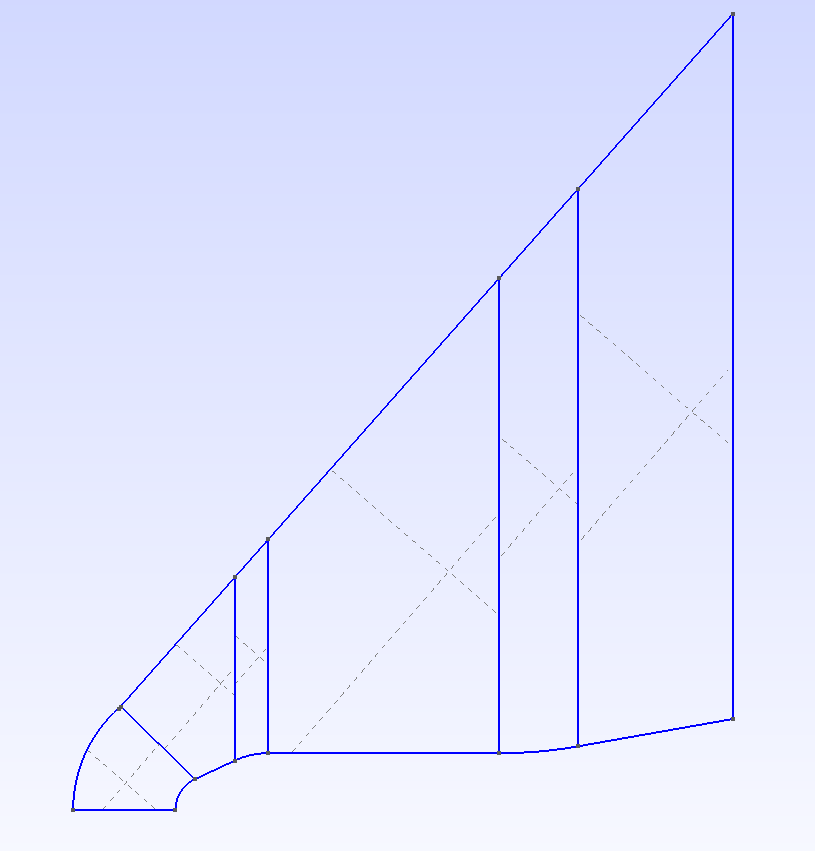
\includegraphics[width=0.5\textwidth]{chapter1_introduction/pictures/gmsh/hb2_geo.png}
\caption{Géométrie HB-2}
\end{center}
\end{figure}

Par la suite je crée les différentes surfaces sur chaque bloc. On veut obtenir un maillage structuré. Il est nécessaire de définir des surfaces à quatre côtés. Si les surfaces ont plus de quatre cotés il sera alors impossible d'utiliser les fonctions dites ‘transfinite’ pour produire un maillage structuré.\\
J'utilise les fonctions 'transfinite curve' sur les différentes droites pour définir le nombre de discrétisations et la progression géométrique des mailles.\\
Pour finir, il faut définir les conditions aux limites, l'amont qui est l'intérieur du domaine, l'aval qui est la sortie, la paroi qui représente l'objet et la droite en amont du HB-2 est définie en tant que symétrie à l'aide des fonctions 'physical line'.\\
Le maillage réalisé et présenté sur les figures suivantes.

Le HB-2 n'est pas très compliqué à mailler,  le domaine est adapté à la géométrie pour obtenir un maillage orthogonal à la paroi.


\begin{figure}[H]
\begin{center}
\begin{subfigure}{0.5\textwidth}
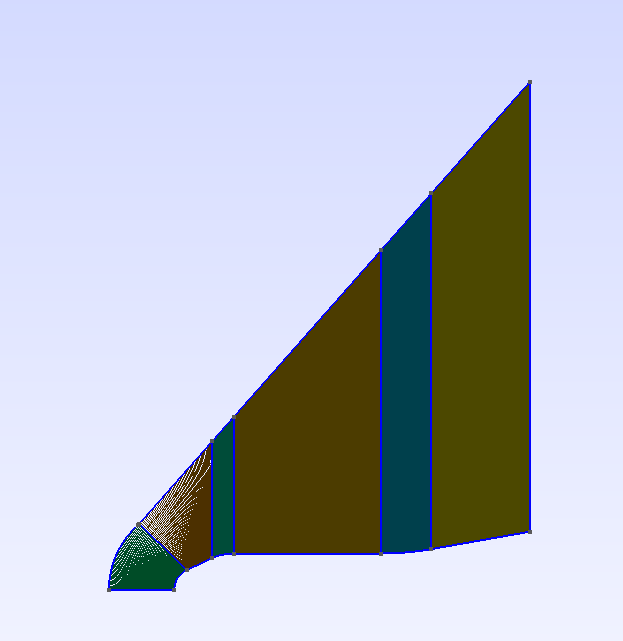
\includegraphics[width=\textwidth]{chapter1_introduction/pictures/gmsh/hb2_mesh1.png}
\end{subfigure}
\begin{subfigure}{0.5\textwidth}
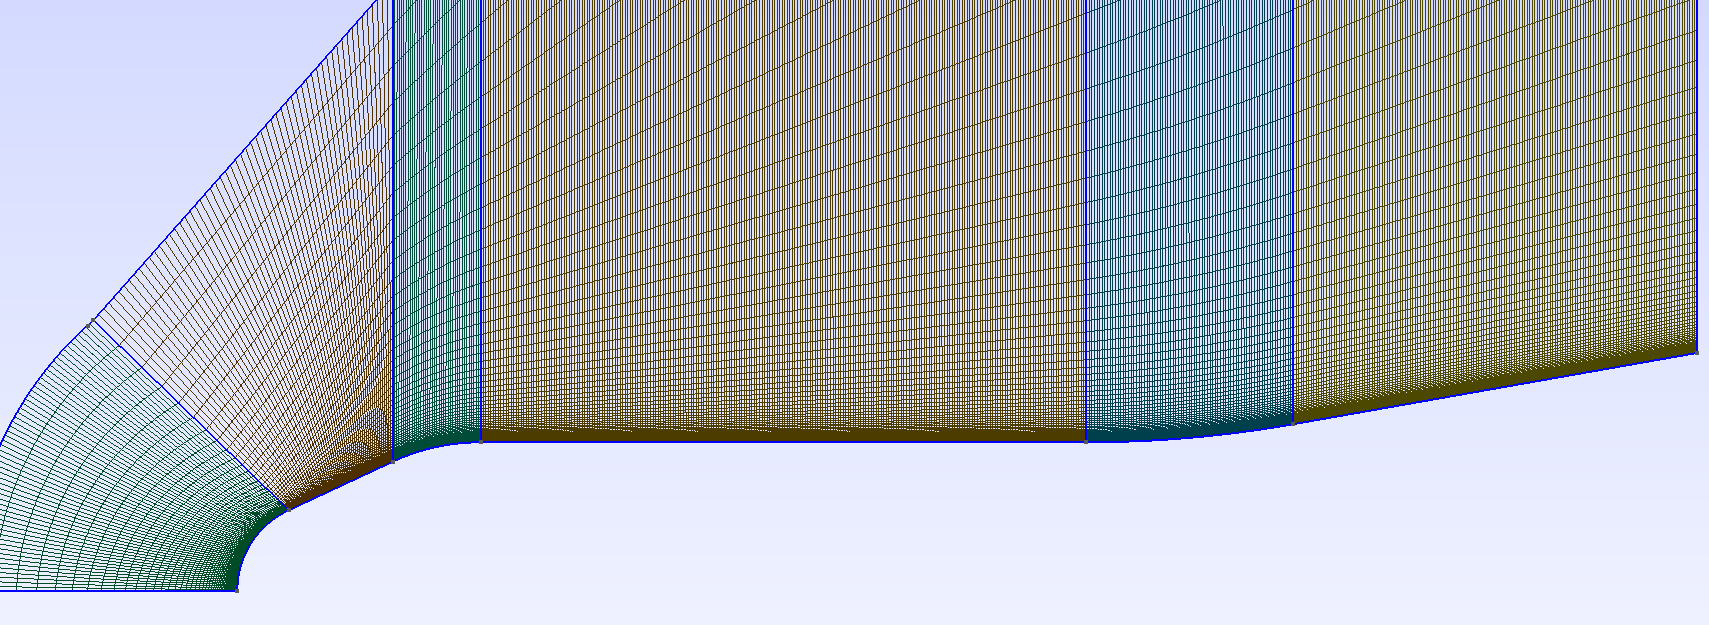
\includegraphics[width=\textwidth]{chapter1_introduction/pictures/gmsh/hb2_mesh2.png}
\end{subfigure}
\begin{subfigure}{0.5\textwidth}
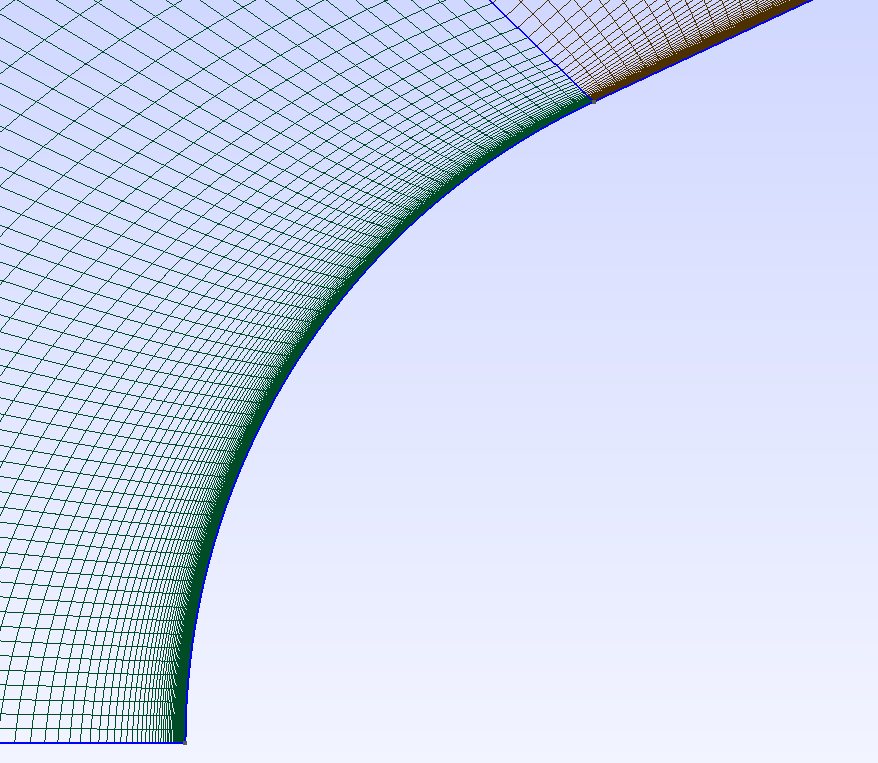
\includegraphics[width=\textwidth]{chapter1_introduction/pictures/gmsh/hb2_mesh3.png}
\end{subfigure}
\caption{Maillage final du HB-2}
\end{center}
\end{figure}
\newpage
\subsubsection{Qualité du maillage}

Une fois le maillage terminé, nous pouvons regarder sa qualité à l'aide de trois critères qui sont 'Gamma',  'SICN' et 'SIGE. Ce sont les seuls critères que le logiciel propose. On les calcule respectivement de la façon suivante:


\begin{equation}
    \gamma = \frac{r_{ci}}{r_{cc}}
\end{equation}

\begin{equation}
    \eta = \frac{V^{\frac{2}{3}}}{\sum l_a^2}
\end{equation}

\begin{equation}
    \epsilon = \frac{minl_a}{maxl_a}
\end{equation}

V représente le volume ou l'aire de l'élément 3D ou 2D, $l_a$ est la longueur d'une arête, $r_{cc}$ est le rayon de la sphère circonscrit en 3D et du cercle circonscrit en 2D, $r_{ci}$ est le rayon de la sphère ou du cercle inscrit en 3D ou en 2D.

Pour le maillage structuré je m'intéresse à deux critères en particulier le 'Gamma' est le 'SIGE'.\\
Plus la valeur de 'Gamma' est proche de 1, plus la qualité du maillage est bonne, si le maillage contient des valeurs avec un faible gamma alors les éléments sont dits distordus et ils vont détériorer les résultats des simulations. Les valeurs pour ce critère sont assez bonnes dans l'ensemble, ils sont compris entre [0.42,1], avec les valeurs les plus basses dans le champ lointain.

Le critère 'SIGE' correspond à la longueur minimum d'une arête d'un élément divisée par la longueur maximale d'une arête du même élément. Après normalisation, plus le critère est proche de 1, meilleur est la qualité du maillage qui permettra d'éviter des erreurs ou des difficultés lors des calculs numériques.

Les valeurs moyennes pour ces deux critères sont répertoriées dans le tableau suivant.

\begin{figure}[H]
\begin{center}
\begin{subfigure}{0.48\textwidth}
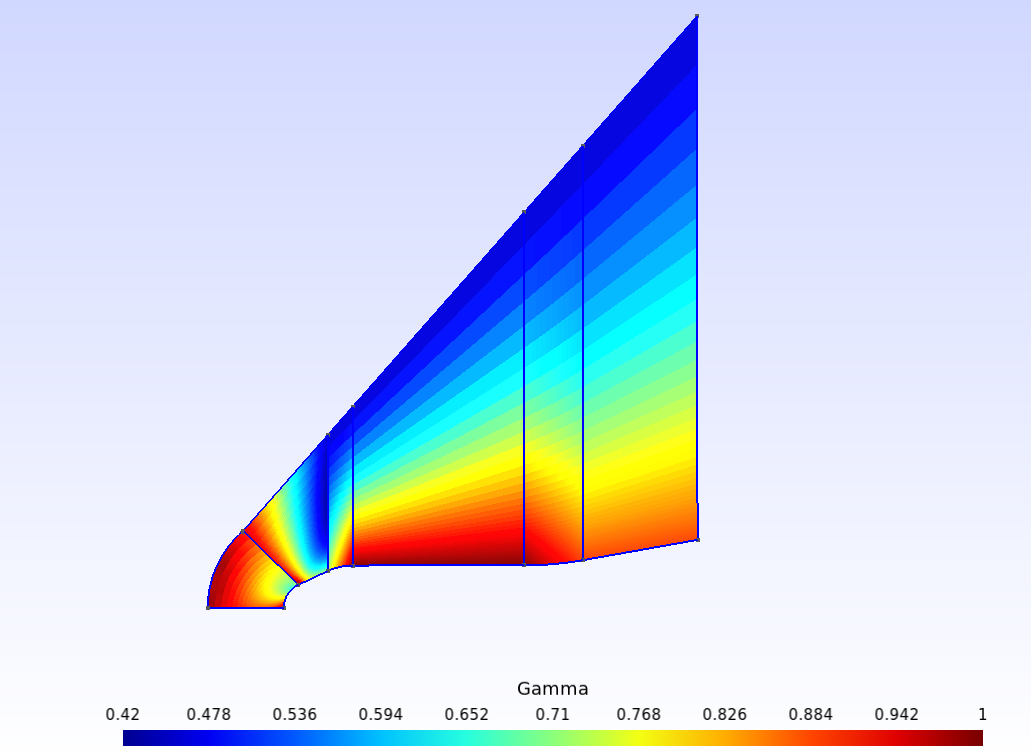
\includegraphics[width=\textwidth]{chapter1_introduction/pictures/gmsh/gamma.png}
\end{subfigure}
\begin{subfigure}{0.48\textwidth}
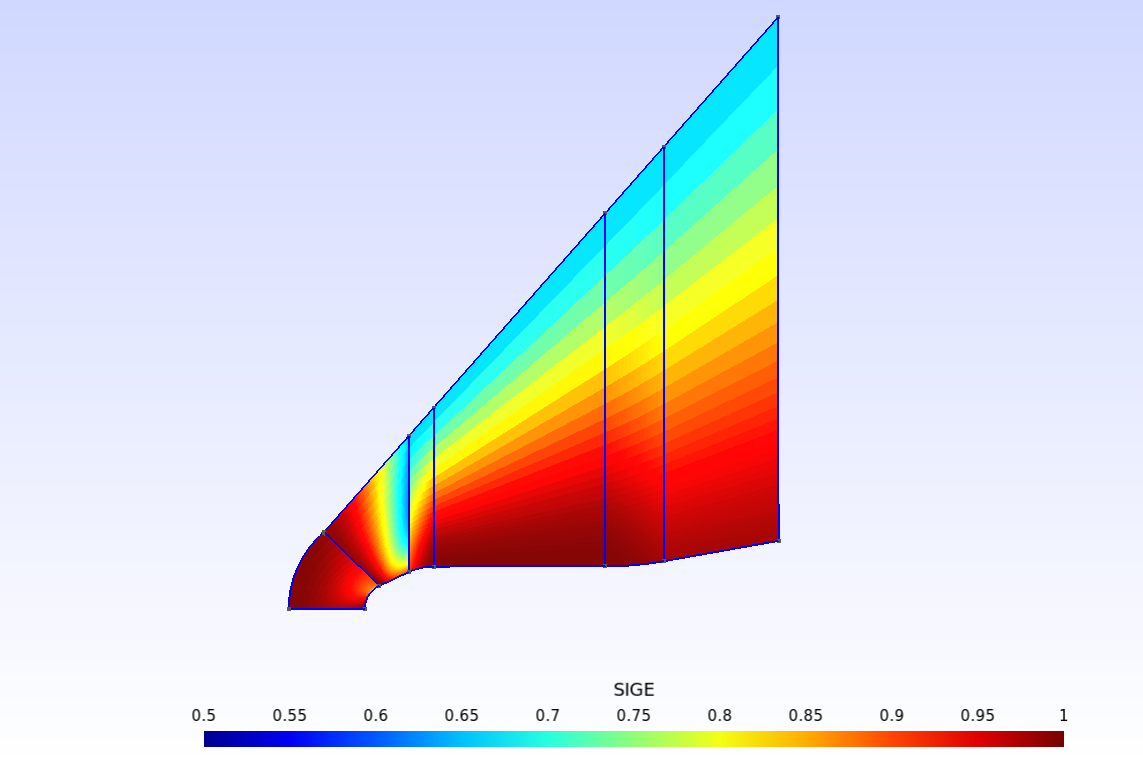
\includegraphics[width=\textwidth]{chapter1_introduction/pictures/gmsh/critere1.png}
\end{subfigure}
\caption{Critére Gamma et SIGE}
\end{center}
\end{figure}

\begin{center}
\begin{tabular}{|c|c|}%3 pour trois colonnes
\hline%ligne horizontale
 Gamma& 0.84 \\%valeur des cases sur une horizontale
\hline
SIGE  &0.92 \\
\hline
\end{tabular}
\captionof{table}{Valeur moyenne de Gamma et SIGE}
\end{center}

\subsection{ICEM}

Le but de mon stage est d'évaluer trois mailleurs entre eux. Lors des trois prochains chapitres nous détaillerons les environnements de travail de chaque mailleur, nous présenterons la réalisation d'un maillage sur logiciel ainsi que leurs critères de qualité. Pour évaluer au mieux ces outils, chaque maillage a été réalisé avec chacun des mailleurs. D’autres cas de comparaison sont aussi en annexe.\\
On commencera par le logiciel actuellement utilisé au sein de CEA/CESTA: ICEM CFD.\\

Le travail réalisé avec ICEM CFD s'est fait sur deux environnements différents. Le début du stage étant en télétravail, j'ai commencé par utiliser ce logiciel sur un environnement Windows.\\
Dès que j'ai pu retourner travailler sur le centre, la suite des travaux sur ICEM s'est faite sur un environnement linux. La version utilisée est la 19.2.\\

ICEM CFD est un mailleur proposé par l'éditeur ANSYS. Ce logiciel de maillage est extrêmement performant pour faire des maillages structurés et non-structurés, que ce soit en deux dimensions ou en trois dimensions.\\
La réalisation de maillage réglé en 2D et 3D se fait essentiellement à l'aide de la méthode multibloc pour obtenir une qualité de maillage élevée.\\
Avec ce logiciel il est facile de mailler des géométries simples pour réaliser un maillage multibloc structuré. Si les géométries deviennent plus complexes on doit employer des méthodes spécifiques aux problèmes avec plusieurs options implémentées au logiciel.\\

Je l‘ai utilisé de façon interactive. C'est à dire que l’on sélectionne les différentes options proposées par le logiciel pour réaliser le maillage mais aussi les géométries si on le souhaite. Cela permet de garder un visuel de la conception du maillage et du blocking réalisé.\\

L'utilisation de ICEM CFD est très difficile, surtout pour la réalisation de maillage multibloc structuré.\\
Pour réaliser un maillage conforme qui soit adapté à la géométrie, il faut procéder en plusieurs étapes et les réaliser dans un ordre bien précis, détaillé à travers l'exemple qui va suivre.\\
De plus pour des géométries en trois dimensions le blocking peut devenir compliqué à produire, il y aura énormément de blocs. Il faut alors réussir à visualiser la subdivision des différents blocs, adapter la géométrie des blocs, bien utiliser les fonctionnalités au risque de ne pas obtenir un maillage structuré.


\section{ Sphère-cône}

L'exemple pris pour le logiciel ICEM CFD est une géométrie composée d'une sphère et d'un cône, où je vais mailler la partie solide de l'objet ainsi que le domaine de calcul. La partie solide comprend une extrusion de matière d'un cône sphère en son centre.\\
Pour construire ce maillage, je commence par importer le fichier Step, qui un fichier de géométrie, comprenant le domaine de calcul ainsi que le solide.\\

Avec ce logiciel il est nécessaire de définir les conditions aux limites dès le début. Je commence par nommer les différentes parties comme l'amont et la paroi.


\begin{figure}[H]
\begin{center}
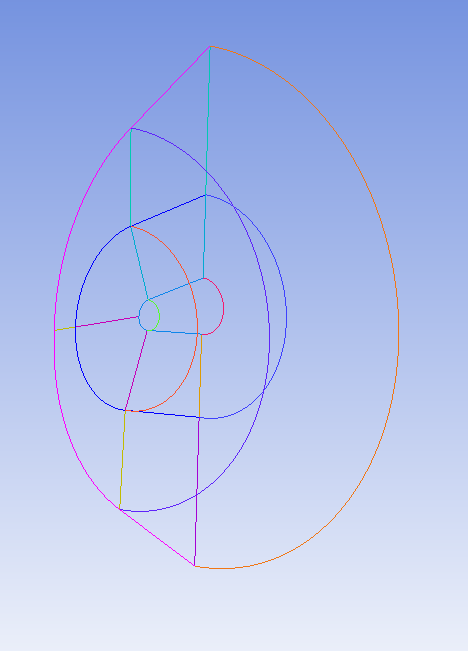
\includegraphics[width=0.45\textwidth]{chapter1_introduction/pictures/icem/castest_fluid_solid/geo1.PNG}
\caption{Géométrie sphère-cône}
\end{center}
\end{figure}

Pour avoir un maillage multibloc avec ICEM, je doi définir un bloc principal qui prend en compte l'intégralité de la géométrie importée, c'est à dire le domaine et l'entité géométrique.\\
Le domaine étant un cône sphère comme la géométrie, je décide d'utiliser la fonction ‘ogird’ pour découper le bloc principal. Cette fonction permet de créer une prézone autour de l'objet en définissant de nouveaux blocs autour de la géométrie.\\

Cette fonction est utilisée à deux reprises, une première fois pour la partie solide et une seconde fois pour la partie fluide.\\

Avec ICEM, il faut faire la différence entre les points, les sommets topologiques, les courbes et les arêtes. Les points et les courbes sont définies par les géométries alors que les sommets topologiques et les arêtes sont définies par la topologie. Il faut associer les courbes et les arêtes qui vont de pair et faire de même entre les sommets topologiques et les points. Une fois que les différentes associations sont faites, je dois supprimer le bloc central qui correspond à l'extrusion de matière.\\



\begin{figure}[H]
\begin{center}
\begin{subfigure}{0.5\textwidth}
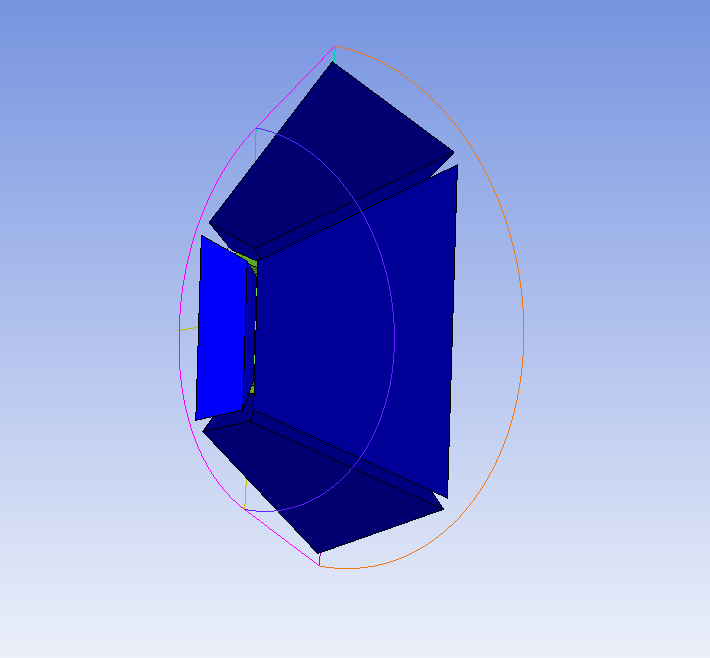
\includegraphics[width=\textwidth]{chapter1_introduction/pictures/icem/castest_fluid_solid/blk1.PNG}
\label{fig:subim1}
\end{subfigure}
\begin{subfigure}{0.5\textwidth}
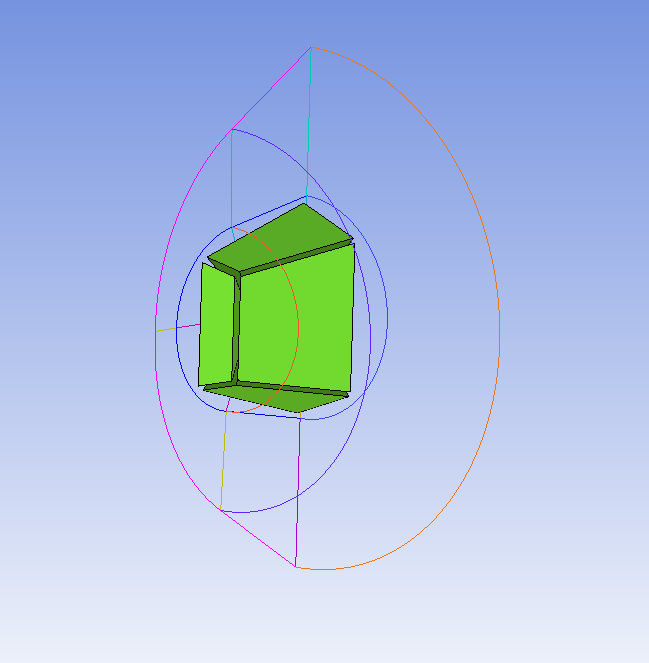
\includegraphics[width=\textwidth]{chapter1_introduction/pictures/icem/castest_fluid_solid/blk2.PNG}
\label{fig:subim2}
\end{subfigure}
\caption{Blocking sphère-cône}
\label{fig:image2}
\end{center}
\end{figure}

Pour finir il faut discrétiser chaque côté avec les fonctions de "sizing". Cette fonction a plusieurs paramètres qui permettent d’introduire du biais si on le souhaite. Il y a le "spacing 1" qui représente la taille de la première maille et le "spacing 2" qui est la taille de la dernière maille sur une courbe.\\
Pour savoir quelle est la première et la dernière maille d’une courbe il y a une flèche qui indique la direction du biais.\\

Pour faire varier le biais, il y a le "ratio 1" et le "ratio 2", que l’on augmente ou diminue pour avoir une progression du maillage.\\
De plus, il y a des fonctions utiles dans ICEM que nous utilisons comme celle qui permet d’avoir la même taille de maille d’un bloc à un autre, pour ne pas avoir de différence de maille inter-bloc.

\begin{figure}[H]
\begin{center}
\begin{subfigure}{0.6\textwidth}
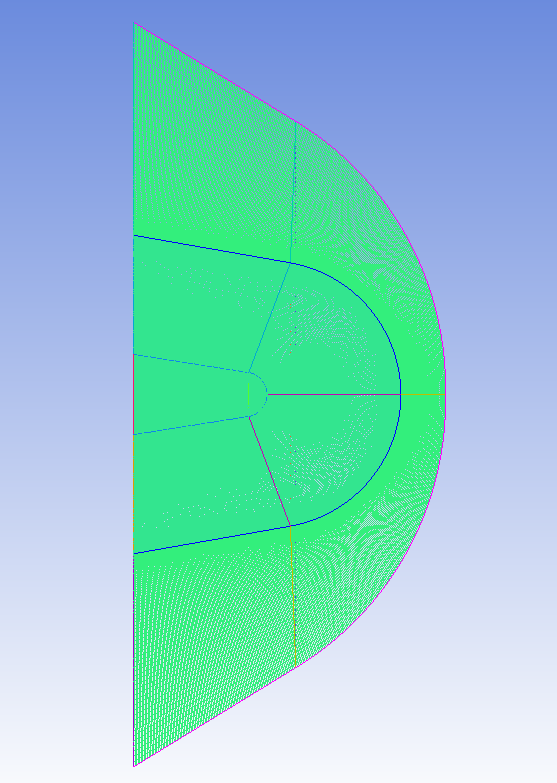
\includegraphics[width=\textwidth]{chapter1_introduction/pictures/icem/castest_fluid_solid/mesh1.PNG}
\label{fig:subim1}
\end{subfigure}
\begin{subfigure}{0.6\textwidth}
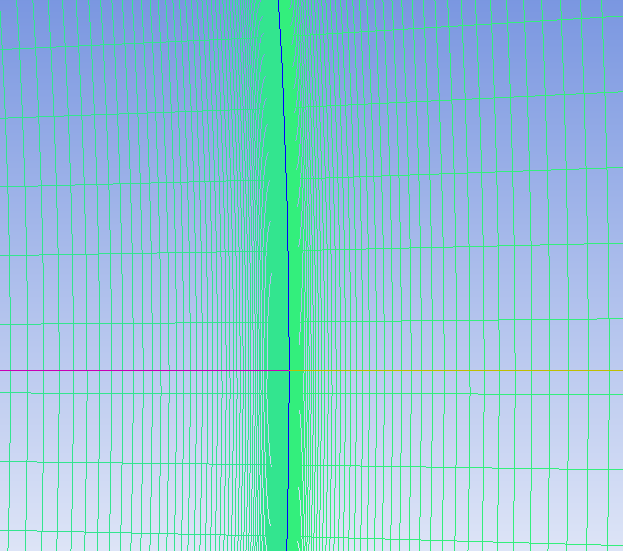
\includegraphics[width=\textwidth]{chapter1_introduction/pictures/icem/castest_fluid_solid/mesh2.PNG}
\label{fig:subim2}
\end{subfigure}
\caption{Maillage final du sphère-cône}
\label{fig:image2}
\end{center}
\end{figure}

\section{ Qualité du maillage}

On peut regarder la qualité d’un maillage à l'aide de certains paramètres. Pour des maillages composés exclusivement d'hexaèdres, les trois principaux critères de qualité sont le déterminant, la distorsion et l'angle.\\
J'ai choisi de regarder deux de ces éléments avec ICEM: le déterminant et l'angle.\\

Le déterminant peut être calculé pour des éléments linéaires hexaédriques, quads et pyramidaux. Sa valeur est calculée à chaque nœud de chaque élément.\\
La valeur du déterminant est comprise entre [0,1]. Un élément du maillage est dit régulier si sa valeur est proche de 1, et il sera dégénéré s’il est proche de 0. Si la valeur est inférieure à 0 alors les éléments sont dits inversés et pourraient compromettre les résultats du calcul numérique.\\
Pour la plupart des solveurs, il faut une valeur supérieure à 0,1. Nos valeurs sont comprises entre [0.8,1], ainsi le maillage sera utilisable par les différents solveurs.


\begin{figure}[H]
\begin{center}
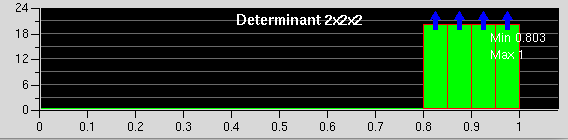
\includegraphics[width=\textwidth]{chapter1_introduction/pictures/icem/castest_fluid_solid/det2.PNG}
\caption{Déterminant 2x2x2}
\end{center}
\end{figure}




L'angle représente les valeurs des angles internes des faces de chaque élément. Ces valeurs sont comprises entre entre 0 et 90 degrés.\\
Ce critère permet de connaître l'aplatissement des cellules qui composent le maillage, plus l'angle est petit et plus la maille sera aplatie et pourra compliquer le calcul par la suite.\\
Pour que le maillage soit utilisable sur les solveurs il faut des valeurs d’angles comprises entre 18 degrés et 90 degrés.


\begin{figure}[H]
\begin{center}
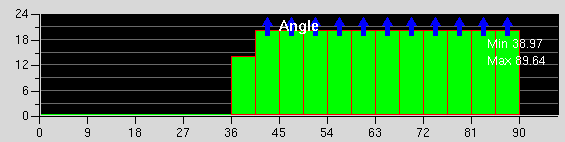
\includegraphics[width=\textwidth]{chapter1_introduction/pictures/icem/castest_fluid_solid/angle.PNG}
\caption{Angle}
\end{center}
\end{figure}


\section {DNS\_LES\_RANS}


\chapter{2: Immersed boundary}

\include{chapter2_immersed_boundary/direct}

\include{chapter2_immersed_boundary/indirect}

\include{chapter2_immersed_boundary/ghost}

\chapter{3: numerical methods}

\section{interpolation}
\subsection{WENO 3}

\begin{equation}
q_{i \pm \frac{1}{2}}^{\mp}=\omega_{0}^{\mp} q_{i \pm \frac{1}{2}}^{(0 \mp)}+\omega_{1}^{\mp} q_{i \pm \frac{1}{2}}^{(1 \mp)}
\end{equation}

\begin{equation}
\begin{array}{ll}
q_{i+\frac{1}{2}}^{(0-)}  =-\frac{1}{2} Q_{i-1}+\frac{3}{2} Q_{i},\quad  q_{i-\frac{1}{2}}^{(0+)}=\frac{1}{2} Q_{i-1}+\frac{1}{2} Q_{i} \\
q_{i+\frac{1}{2}}^{(1-)}  =\frac{1}{2} Q_{i}+\frac{1}{2} Q_{i+1}, \quad q_{i-\frac{1}{2}}^{(1+)}=\frac{3}{2} Q_{i}-\frac{1}{2} Q_{i+1} .
\end{array}
\end{equation}

\begin{equation}
\begin{array}{l}
I S_{0}=\left(Q_{i}-Q_{i-1}\right)^{2} \\
I S_{1}=\left(Q_{i+1}-Q_{i}\right)^{2}
\end{array}
\end{equation}

with $\gamma_{0}^{-}=\gamma_{1}^{+}=\frac{1}{3}, \gamma_{1}^{-}=\gamma_{0}^{+}=\frac{2}{3}$ and $\tau_{3}=\left|I S_{0}-I S_{1}\right| .$ The $\epsilon$ is a
small positive number used to avoid division by zero. We set $\epsilon=\Delta x^{4}$. The description is now complete. We refer to this reconstruction method as WENO-Z3.

\subsection{WENO 5}

\begin{equation}
\begin{array}{ll}
q_{i+\frac{1}{2}}^{(0-)}  =\frac{1}{3} Q_{i-2}-\frac{7}{6} Q_{i-1}+\frac{11}{6} Q_{i},\quad  q_{i+\frac{1}{2}}^{(0+)}=-\frac{1}{6} Q_{i-1}+\frac{5}{6} Q_{i}+\frac{1}{3} Q_{i+1} \\
q_{i+\frac{1}{2}}^{(1-)}  =-\frac{1}{6} Q_{i-1}+\frac{5}{6} Q_{i}+\frac{1}{3} Q_{i+1}, \quad  q_{i+\frac{1}{2}}^{(1+)}=\frac{1}{3} Q_{i}+\frac{5}{6} Q_{i+1}-\frac{1}{6} Q_{i+2} \\
q_{i+\frac{1}{2}}^{(2-)}  =\frac{1}{3} Q_{i}+\frac{5}{6} Q_{i+1}-\frac{1}{6} Q_{i+2}, \quad q_{i-\frac{1}{2}}^{(2+)}=\frac{11}{6} Q_{i+1}-\frac{7}{6} Q_{i+2}+\frac{1}{3} Q_{i+3}
\end{array}
\end{equation}

\begin{equation}
\begin{array}{l}
q_{i+\frac{1}{2}}^{-}=\omega_{0}^{-} q_{i+\frac{1}{2}}^{(1-)}+\omega_{1}^{-} q_{i+\frac{1}{2}}^{(2-)}+\omega_{2}^{-} q_{i+\frac{1}{2}}^{(3-)} \\
q_{i+\frac{1}{2}}^{+}=\omega_{0}^{+} q_{i+\frac{1}{2}}^{(1+)}+\omega_{1}^{+} q_{i+\frac{1}{2}}^{(2+)}+\omega_{2}^{+} q_{i+\frac{1}{2}}^{(3+)}
\end{array}
\end{equation}

\begin{equation}
\begin{array}{l}
I S_{0}=\frac{13}{12}\left(Q_{i-2}-2 Q_{i-1}+Q_{i}\right)^{2}+\frac{1}{4}\left(Q_{i-2}-4 Q_{i-1}+3 Q_{i}\right)^{2} \\
I S_{1}=\frac{13}{12}\left(Q_{i-1}-2 Q_{i}+Q_{i+1}\right)^{2}+\frac{1}{4}\left(Q_{i-1}+Q_{i+1}\right)^{2} \\
I S_{2}=\frac{13}{12}\left(Q_{i}-2 Q_{i+1}+Q_{i+2}\right)^{2}+\frac{1}{4}\left(3 Q_{i}-4 Q_{i+1}+Q_{i+2}\right)^{2}
\end{array}
\end{equation}

\begin{equation}
\omega_{k}^{\pm}=\frac{\bar{\omega}_{k}^{\pm}}{\tilde{\omega}_{0}^{\pm}+\tilde{\omega}_{1}^{\pm}+\tilde{\omega}_{2}^{\pm}}, \quad \tilde{\omega}_{k}^{\pm}=\frac{\gamma_{k}^{\pm}}{\left(\epsilon+I S_{k}\right)^{p}}, \quad k=0,1,2
\end{equation}


$$
\omega_{k}^{\pm}=\frac{\tilde{\omega}_{k}^{\pm}}{\tilde{\omega}_{0}^{\pm}+\tilde{\omega}_{1}^{\pm}+\tilde{\omega}_{2}^{\pm}}, \quad \tilde{\omega}_{k}^{\pm}=\gamma_{k}^{\pm}\left(1+\left(\frac{\tau_{5}}{I S_{k}+\epsilon}\right)^{p}\right), \quad k=0,1,2
$$
with $\tau_{5}=\left|I S_{0}-I S_{2}\right|, \epsilon=\Delta x^{4}, p=2,$ and $\gamma_{k}^{\pm}$ as above.

\subsection{WENO 7}

\begin{equation}
q_{i \pm \frac{1}{2}}^{(k \mp)}=\sum_{l=0}^{3} a_{k, l}^{\pm} Q_{i-3+k+l}
\end{equation}

\begin{equation}
\begin{array}{c||cccc}
l & 0 & 1 & 2 & 3 \\
\hline a_{0, l}^{+} & \frac{-3}{12} & \frac{13}{12} & \frac{-23}{12} & \frac{25}{12} \\
a_{1, l}^{+} & \frac{1}{12} & \frac{-5}{12} & \frac{13}{12} & \frac{3}{12} \\
a_{2, l}^{+} & \frac{-1}{12} & \frac{7}{12} & \frac{7}{12} & \frac{-1}{12} \\
a_{3, l}^{+} & \frac{3}{12} & \frac{13}{12} & \frac{-5}{12} & \frac{1}{12}
\end{array}
\end{equation}

\begin{equation}
\begin{array}{ll}
q_{i+\frac{1}{2}}^{(0-)}  =\frac{1}{3} Q_{i-2}-\frac{7}{6} Q_{i-1}+\frac{11}{6} Q_{i},\quad  q_{i+\frac{1}{2}}^{(0+)}=-\frac{1}{6} Q_{i-1}+\frac{5}{6} Q_{i}+\frac{1}{3} Q_{i+1} \\
q_{i+\frac{1}{2}}^{(1-)}  =-\frac{1}{6} Q_{i-1}+\frac{5}{6} Q_{i}+\frac{1}{3} Q_{i+1}, \quad  q_{i+\frac{1}{2}}^{(1+)}=\frac{1}{3} Q_{i}+\frac{5}{6} Q_{i+1}-\frac{1}{6} Q_{i+2} \\
q_{i+\frac{1}{2}}^{(2-)}  =\frac{1}{3} Q_{i}+\frac{5}{6} Q_{i+1}-\frac{1}{6} Q_{i+2}, \quad q_{i-\frac{1}{2}}^{(2+)}=\frac{11}{6} Q_{i+1}-\frac{7}{6} Q_{i+2}+\frac{1}{3} Q_{i+3}
\end{array}
\end{equation}

\begin{equation}
\begin{array}{c}
I S_{0}=Q_{i-3}\left(547 Q_{i-3}-3882 Q_{i-2}+4642 Q_{i-1}-1854 Q_{i}\right)+ \\
\quad Q_{i-2}\left(7043 Q_{i-2}-17246 Q_{i-1}+7042 Q_{i}\right)+ \\
\quad Q_{i-1}\left(11003 Q_{i-1}-9402 Q_{i}\right)+2107 Q_{i}^{2} \\
I S_{1}=  Q_{i-2}\left(267 Q_{i-2}-1642 Q_{i-1}+1602 Q_{i}-494 Q_{i+1}\right)+ \\
Q_{i-1}\left(2843 Q_{i-1}-5966 Q_{i}+1922 Q_{i+1}\right)+ \\
Q_{i}\left(3443 Q_{i}-2522 Q_{i+1}\right)+547 Q_{i+1}^{2}, \\
I S_{2}=  Q_{i-1}\left(547 Q_{i-1}-2522 Q_{i}+1922 Q_{i+1}-494 Q_{i+2}\right)+ \\
Q_{i}\left(3443 Q_{i}-5966 Q_{i+1}+1602 Q_{i+2}\right)+ \\
Q_{i+1}\left(2843 Q_{i+1}-1642 Q_{i+2}\right)+267 Q_{i+2}^{2}, \\
IS_{3}=  Q_{i}\left(2107 Q_{i}-9402 Q_{i+1}+7042 Q_{i+2}-1854 Q_{i+3}\right)+ \\
Q_{i+1}\left(11003 Q_{i+1}-17246 Q_{i+2}+4642 Q_{i+3}\right)+ \\
Q_{i+2}\left(7043 Q_{i+2}-3882 Q_{i+3}\right)+547 Q_{i+3}^{2}
\end{array}
\end{equation}

\begin{equation}
\begin{array}{l}
\text { with } \gamma_{0}^{-}=\gamma_{3}^{+}=\frac{1}{35}, \gamma_{1}^{-}=\gamma_{2}^{+}=\frac{12}{35}, \gamma_{2}^{-}=\gamma_{1}^{+}=\frac{18}{35}, \gamma_{3}^{-}=\gamma_{0}^{+}=\frac{4}{35}, \epsilon=\Delta x^{2} \\
\text { and } p=2
\end{array}
\end{equation}

\subsection{TENO 5}

\begin{equation}
\begin{array}{l}
\hat{f}_{0, i+1 / 2}=\frac{1}{6}\left(-f_{i-1}+5 f_{i}+2 f_{i+1}\right) \\
\hat{f}_{1, i+1 / 2}=\frac{1}{6}\left(2 f_{i}+5 f_{i+1}-f_{i+2}\right) \\
\hat{f}_{2, i+1 / 2}=\frac{1}{6}\left(2 f_{i-2}-7 f_{i-1}+11 f_{i}\right)
\end{array}
\end{equation}

\begin{equation}
\begin{array}{l}
\hat{f}_{3, i+1 / 2}=\frac{1}{12}\left(3 f_{i}+13 f_{i+1}-5 f_{i+2}+f_{i+3}\right) \\
\hat{f}_{4, i+1 / 2}=\frac{1}{12}\left(-3 f_{i-3}+13 f_{i-2}-23 f_{i-1}+25 f_{i}\right) \\
\hat{f}_{5, i+1 / 2}=\frac{1}{60}\left(12 f_{i}+77 f_{i+1}-43 f_{i+2}+17 f_{i+3}-3 f_{i+4}\right)
\end{array}
\end{equation}

\subsection{TENO 7}

\begin{equation}
\begin{aligned}
\beta_{0,3} &=\frac{1}{4}\left(f_{i-1}-f_{i+1}\right)^{2}+\frac{13}{12}\left(f_{i-1}-2 f_{i}+f_{i+1}\right)^{2} \\
\beta_{1,3} &=\frac{1}{4}\left(3 f_{i}-4 f_{i+1}+f_{i+2}\right)^{2}+\frac{13}{12}\left(f_{i}-2 f_{i+1}+f_{i+2}\right)^{2} \\
\beta_{2,3} &=\frac{1}{4}\left(f_{i-2}-4 f_{i-1}+3 f_{i}\right)^{2}+\frac{13}{12}\left(f_{i-2}-2 f_{i-1}+f_{i}\right)^{2} \\
\beta_{3,4} &=\frac{1}{240}\left[f_{i}\left(2107 f_{i}-9402 f_{i+1}+7042 f_{i+2}-1854 f_{i+3}\right)\right.\\
&+f_{i+1}\left(11003 f_{i+1}-17246 f_{i+2}+4642 f_{i+3}\right) \\
&\left.+f_{i+2}\left(7043 f_{i+2}-3882 f_{i+3}\right)+547 f_{i+3} f_{i+3}\right] \\
\beta_{4,4} &=\frac{1}{240}\left[f_{i-3}\left(547 f_{i-3}-3882 f_{i-2}+4642 f_{i-1}-1854 f_{i}\right)\right.\\
&+f_{i-2}\left(7043 f_{i-2}-17246 f_{i-1}+7042 f_{i}\right) \\
&\left.+f_{i-1}\left(11003 f_{i-1}-9402 f_{i}\right)+2107 f_{i} f_{i}\right]
\end{aligned}
\end{equation}

\begin{equation}
\gamma_{k}=\left(C+\frac{\tau_{K}}{\beta_{k, r_{k}}+\varepsilon}\right)^{q}, k=0, \ldots, K-3
\end{equation}

\begin{equation}
\beta_{k, r_{k}}=\sum_{j=1}^{r-1} \Delta x^{2 j-1} \int_{x_{i-1 / 2}}^{x_{i+1 / 2}}\left(\frac{d^{j}}{d x^{j}} \hat{f}_{k}(x)\right)^{2} d x
\end{equation}

\begin{equation}
\tau_{K}=\left|\beta_{K}-\frac{1}{6}\left(\beta_{1,3}+\beta_{2,3}+4 \beta_{0,3}\right)\right|=O\left(\Delta x^{6}\right)
\end{equation}

\begin{equation}
\chi_{k}=\frac{\gamma_{k}}{\sum_{k=0}^{K-3} \gamma_{k}}
\end{equation}

\begin{equation}
\delta_{k}=\left\{\begin{array}{ll}
0, & \text { if } \chi_{k}<C_{T} \\
1, & \text { otherwise }
\end{array}\right.
\end{equation}

\begin{figure}[H]
\begin{center}
        \includegraphics[width=\textwidth]{shémas de descretisation/castest/photo/tenoweno.PNG}
\caption{}
\end{center}
\end{figure}


\section{Riemann problem}

On appelle problème de Riemann pour les équations d'Euler monodimensionnelles le problème consistant à chercher une solution des équations avec la condition initiale suivante :
\begin{equation}
\frac{\partial \vec{U}}{\partial t}+\frac{\partial \vec{F}}{\partial x}=\overrightarrow{0} \quad ; \quad \vec{U}(x, 0)=\vec{U}^{0}(x)=\left\{\begin{array}{lll}
\vec{U}_{L} & \text { si } & x<0 \\
\vec{U}_{R} & \text { si } & x>0
\end{array}\right.
\end{equation}
\subsection{equation noninéarire}
Dans cette partie nous allonsnous interreeser au prebleme de Riemann pour les equation non lieair ainsi que pour les ss teme n0n lineaire. Nous detailerons les different phenomeme que nous puvons rencontre lors de la resolutions d'n probleme de riemann nonlineaire. L'equation non lineaire que nous allons prendre en exemple et l'équation de burguers:
\begin{equation}
\frac{\partial u}{\partial t}+\frac{\partial f(u)}{\partial x}=0 \quad ; \quad f(u)=\frac{u^{2}}{2} \quad ; \quad u(x, 0)=u^{0}(x)
\end{equation}

\begin{equation}
u^{0}(x)=\left\{\begin{array}{lll}
u_{L} & \text { si } & x<0 \\
u_{R} & \text { si } & x>0
\end{array}\right.
\end{equation}

Les conditions initiales sont
- compressives si $u_{L}>u_{R} \rightarrow$ formation d'un choc expansives $\quad$ si $u_{L}<u_{R} \rightarrow$ formation d'un éventail de détente

\begin{equation}
\begin{aligned}
&\text { Cl compressives: }\\
&u(x, t)=\left\{\begin{array}{lll}
u_{L} & \text { si } & x / t<S \\
u_{R} & \text { si } & x / t>S
\end{array}\right.\\
&S=\frac{1}{2}\left(u_{L}+u_{R}\right)
\end{aligned}
\end{equation}

\begin{equation}
\begin{aligned}
&\text { CI expansives }\\
&u(x, t)=\left\{\begin{array}{ccl}
u_{L} & \text { si } & x / t<u_{L} \\
x / t & \text { si } & u_{L}<x / t<u_{R} \\
u_{R} & \text { si } & x / t>u_{R}
\end{array}\right.
\end{aligned}
\end{equation}
\begin{figure}[H]
\begin{center}
\includegraphics[width=0.6\textwidth]{solveur de Rieamman/photo/riemann.PNG}
\caption{}
\end{center}
\end{figure}
\begin{figure}[H]
\begin{center}
        \includegraphics[width=0.6\textwidth]{solveur de Rieamman/photo/riemann.PNG}
\caption{}
\end{center}
\end{figure}
\begin{figure}[H]
\begin{center}
        \includegraphics[width=0.6\textwidth]{solveur de Rieamman/photo/riemann.PNG}
\caption{}
\end{center}
\end{figure}
Ces solutions présentent une similitude en fonction du rapport $\xi=x / t .$ Dans le cas d'un choc (figure $4.4$ ), la discontinuité initiale se propage à vitesse constante $S=\frac{1}{2}\left(u_{L}+u_{R}\right)$ définie par la condition de Rankine-Hugoniot. Dans le cas de la détente (figure 4.5), la solution est une droite reliant le pied de l'éventail avançant à vitesse $u_{L}$ et la tête de l'éventail avançant à vitesse $u_{R}>u_{L}$


%La solution possède une propriété d'auto-similitude car elle ne dépend que du rapport x/t.
%On montre que la solution est constituée par au plus quatre zones dans lesquelles w est
%constant, séparées par des ondes centrées c'est-à-dire des zones où w est fonction de x/t.
%Eventuellement le nombre de régions peut être réduit à trois auquel cas la région centrale
%est une zone de vide notée (V).

%Ces ondes centrées peuvent être de trois types :
%• Des faisceaux de détente isentropique notés (D) dans lesquels w(x, t) est continue.
%• Des discontinuités de contact à travers lesquelles la pression et la vitesse sont continues et seule la densité est discontinue. On appelle ces discontinuités lignes de glissement notées (L).
%• Des discontinuités de type ondes de choc notées (C) à travers lesquelles w(x, t) est
%discontinue.
%Suivant les valeurs du rapport pL
%pR
%et de la diérence de vitesse uL − uR, il existe cinq
%congurations possibles notées (de gauche à droite) DLC, CLC, CLD, DLD et DVD.
%Certains schémas numériques reposent sur la résolution d'un problème de Riemann à
%chaque interface de calcul, c'est-à-dire la détermination de la solution à chaque interface
%16
%de calcul à partir des états gauche et droit.

\subsection{system equation noninéarire}

Dans le cas général d'un système non-linéaire de $m$ équations, l'état initial discontinu peut-être à l'origine :
de détentes, i.e. d'ondes simples centrées à l'origine pour les champs VNL (équation $(2.82)$ et figure $2.10$ gauche $),$ dont les caractéristiques divergent $\left(\lambda^{(i)}\left(\vec{U}_{L}\right)<\lambda^{(i)}\left(\vec{U}_{R}\right)\right)$ et dont les $i$ -invariants de Riemann faibles sont donnés par $(2.73)$. de discontinuités de contact pour les champs LD, dont les caractéristiques sont des droites parallèles de pente $\lambda^{(i)}\left(\vec{U}_{L}\right)=\lambda^{(i)}\left(\vec{U}_{R}\right)$ (figure $2.11$ droite $)$ qui est la vitesse de propagation de la discontinuité satisfaisant les relations de Rankine-Hugoniot $(2.85)$. Les $i$ -invariants de Riemann faibles vérifient également $(2.73)$ à travers la discontinuité de contact. de chocs pour les champs VNL si $\lambda^{(i)}\left(\vec{U}_{L}\right)>\lambda^{(i)}\left(\vec{U}_{R}\right) .$ Dans ce cas, la vitesse $\mathrm{du}$ choc doit vérifier les relations de Rankine-Hugoniot $(2.85)$ et la condition entropique
$$
\lambda^{(i)}\left(\vec{U}_{L}\right)>S^{(i)}>\lambda^{(i)}\left(\vec{U}_{R}\right)
$$
Chacune de ces solutions d'ondes élémentaires présente une similitude en fonction $\mathrm{du}$ rapport $\xi=x / t$. Il en est donc de même pour la solution du problème de Riemann en général, qui est constitué de $\vec{U}_{L}$ à gauche de l'onde la plus lente, de $(m-1)$ états intermédiaires séparés par l'une quelconque de ces ondes élémentaires, et de $\vec{U}_{R}$ à droite de l'onde la plus rapide.

\subsection{RUSANOV}

Davis made some observations regarding the relationship between the chosen wave speeds and some well-known numerical methods. Suppose that for a given Riemann problem we can identify a positive speed $S^{+}$. Then by choosing $S_{L}=-S^{+}$ and $S_{R}=S^{+}$ in the HLL flux (10.20) one obtains a Rusanov flux [418]
$$
\mathbf{F}_{i+1 / 2}=\frac{1}{2}\left(\mathbf{F}_{L}+\mathbf{F}_{R}\right)-\frac{1}{2} S^{+}\left(\mathbf{U}_{R}-\mathbf{U}_{L}\right)
$$
As to the choice of the speed $S^{+},$ Davis [150] considered
$$
S^{+}=\max \left\{\left|u_{L}-a_{L}\right|,\left|u_{R}-a_{R}\right|,\left|u_{L}+a_{L}\right|,\left|u_{R}+a_{R}\right|\right\}
$$
Actually, the above speed is bounded by
$$
S^{+}=\max \left\{\left|u_{L}\right|+a_{L},\left|u_{R}\right|+a_{R}\right\}
$$
This choice is likely to produce a more robust scheme and is also simpler than Davis's choice.

Another possible choice is $S^{+}=S_{\max }^{n},$ the maximum wave speed present at the appropriate time found by imposing the Courant stability condition; see Sect. 6.3 .2 of Chap. $6 .$ This speed is related to the time step $\Delta t$ and the grid spacing $\Delta x$ via
$$
S_{\max }^{n}=\frac{C_{c f l} \Delta x}{\Delta t}
$$
where $C_{c f l}$ is the Courant number coefficient, usually chosen (empirically) to be $C_{c f l} \approx 0.9,$ for a scheme of linear stability limit of unity. For $C_{c f l}=1$ one has $S^{+}=\frac{\Delta x}{\Delta t},$ which results in the Lax-Friedrichs numerical flux
$$
F_{i+1 / 2}=\frac{1}{2}\left(F_{L}+F_{R}\right)-\frac{1}{2} \frac{\Delta x}{\Delta t}\left(U_{R}-U_{L}\right)
$$

\subsection{HLLC}

La simplicité du schéma HLL est due la représentation a 2 ondes de la solution du problème de Riemann local, qui ne prend pas en considération les ondes LD, de type discontinuité de contact. Ces dernières sont donc mal représentées dans les solutions numériques (voir figure 8.13, section 8.4). Pour y remédier, Toro et al $^{6}$ introduisent une $3^{\text {ème }}$ onde de vitesse $S^{*}$ dans structure du problème (figure 8.7).
FiGure 8.7 - Structure a 3 ondes et 4 états constants du schéma HLLC.
On sépare en deux contributions l'intégrale au membre de gauche de (8.32) :
En posant
$$
\vec{U}_{L}^{*}=\frac{1}{T\left(S^{*}-S_{L}\right)} \int_{T S_{L}}^{T S^{*}} \vec{U}(x, T) d x \quad ; \quad \vec{U}_{R}^{*}=\frac{1}{T\left(S_{R}-S^{*}\right)} \int_{T S^{*}}^{T S_{R}} \vec{U}(x, T) d x
$$
la relation de consistence (8.31) devient
$$
\left(\frac{S^{*}-S_{L}}{S_{R}-S_{L}}\right) \vec{U}_{L}^{*}+\left(\frac{S_{R}-S^{*}}{S_{R}-S_{L}}\right) \vec{U}_{R}=\vec{U}^{H L L}
$$
et les conditions Rankine-Hugoniot (8.35)(8.36) au travers des 3 ondes sont maintenant
$$
\begin{aligned}
\vec{F}_{L}^{*} &=\vec{F}_{L}+S_{L}\left(\vec{U}_{L}^{*}-\vec{U}_{L}\right) \\
\vec{F}_{R} &=\vec{F}_{L}^{*}+S^{*}\left(\vec{U}_{R}^{*}-\vec{U}_{L}^{*}\right) \\
\vec{F}_{R}^{*} &=\vec{F}_{R}+S_{R}\left(\vec{U}_{R}^{*}-\vec{U}_{R}\right)
\end{aligned}
$$
On vérifie aisément qu'en injectant (8.42) et (8.44) dans $(8.43),$ on retrouve $(8.41) .$ On a
problème de Riemann a conduit aux relations (4.16), et il est tout à fait justifié de prendre $S^{*}=u^{*},$ que l'on suppose connu et qu'on déterminera plus tard. On a donc:
ro
M. Speares W., 1994, Restomtion of the contact surface in the HLL-Riemann solver. Shock Waves, vol. $4,$ pp. $25-34$

On récrit (8.42) en passant au membre de droite les grandeurs connues :
$$
S_{L} \vec{U}_{L}^{*}-\vec{F}_{L}^{*}=S_{L} \vec{U}_{L}-\vec{F}_{L}=\vec{Q}_{L} \text { connu }
$$
La relation (3.39) permet d'écrire (8.46) sous la forme
$$
\left(S_{L}-u^{*}\right) \vec{U}_{L}^{*}=p^{*} \vec{D}^{*}+\left(S_{L}-u_{L}\right) \vec{U}_{L}-p_{L} \vec{D}_{L}
$$
Détaillons maintenant les deux premières composantes de (8.42)
$$
\left\{\begin{aligned}
\rho_{L}^{*} u^{*} &=\rho_{L} u_{L} \quad+S_{L}\left(\rho_{L}^{*}-\rho_{L}\right) \\
\rho_{L}^{*} u^{* 2}+p^{*} &=\rho_{L} u_{L}^{2}+p_{L}+S_{L}\left(\rho_{L}^{*} u^{*}-\rho_{L} u_{L}\right)
\end{aligned}\right.
$$
On déduit de la première:
$$
\rho_{L}^{*}\left(u^{*}-S_{L}\right)=\rho_{L}\left(u_{L}-S_{L}\right)
$$
que l'on substitue dans la seconde pour obtenir
$$
p^{*}=p_{L}+\rho_{L}\left(S_{L}-u_{L}\right)\left(u^{*}-u_{L}\right)
$$
que l'on injecte dans (8.48) , ce qui détermine complètement l'écat $\vec{U}_{L}^{*}$. En en détaillant les composantes, on trouve
$$
\vec{U}_{L}=\rho_{L}\left(\frac{S_{L}-u_{L}}{S_{L}-u^{*}}\right) \mid \begin{array}{l}
1 \\
u^{*} \\
E_{L}+\left(u^{*}-u_{L}\right)\left[u^{*}+\frac{p_{L}}{\rho_{L}\left(S_{L}-u_{L}\right)}\right]
\end{array}
$$
où $u^{*}=S^{*}$. En procédent de même a partir de (8.44) , on obtient
$$
\vec{U}_{R}=\rho_{L}\left(\frac{S_{R}-u_{R}}{S_{R}-u^{*}}\right) \mid \begin{array}{l}
1 \\
u^{*} \\
E_{R}+\left(u^{*}-u_{R}\right)\left[u^{*}+\frac{p_{R}}{\rho_{R}\left(S_{R}-u_{R}\right)}\right]
\end{array}
$$
Au final, le flux numérique à l'interface $i+1 / 2$ est
$$
\vec{F}_{i+1 / 2}^{H L L C}=\left\{\begin{array}{ll}
\vec{F}_{L} & \text { si } 0 \leq S_{L} \\
\vec{F}_{L}^{*}=\vec{F}_{L}+S_{L}\left(\vec{U}_{L}^{*}-\vec{U}_{L}\right) & \text { si } S_{L} \leq 0 \leq S^{*} \\
\vec{F}_{R}^{*}=\vec{F}_{R}+S_{R}\left(\vec{U}_{R}^{*}-\vec{U}_{R}\right) & \text { si } S^{*} \leq 0 \leq S_{R} \\
\vec{F}_{R} & \text { si } S_{R} \leq 0
\end{array}\right.
$$
où l'état $L$ est celui de la cellule $I_{i}$ et l'écat $R$ celui de la cellule $I_{i+1}$.
En écrivant (8.50) coté $R$, avec les relations (8.45) , on obtient l'estimation de la vitesse $S^{*}:$
$$
S^{*}=\frac{p_{R}-p_{L}+\rho_{L} u_{L}\left(S_{L}-u_{L}\right)-\rho_{R} u_{R}\left(S_{R}-u_{R}\right)}{\rho_{L}\left(S_{L}-u_{L}\right)-\rho_{R}\left(S_{R}-u_{R}\right)}
$$
Les vitesses $S_{L}$ et $S_{R}$ sont estimées de la même façon que pour le schéma HLL.

\subsection{HLL}

We are concerned with solving numerically the general Initial Boundary Value Problem (IBVP)
$$
\left.\begin{array}{l}
\text { PDEs: } \mathbf{U}_{t}+\mathbf{F}(\mathbf{U})_{x}=\mathbf{0} \\
\text { ICs }: \mathbf{U}(x, 0)=\mathbf{U}^{(0)}(x), \\
\text { BCs }: \mathbf{U}(0, t)=\mathbf{U}_{1}(t), \mathbf{U}(L, t)=\mathbf{U}_{\mathrm{r}}(t),
\end{array}\right\}
$$
in a domain $0 \leq x \leq L,$ with appropriate boundary conditions. We use the explicit conservative formula
$$
\mathbf{U}_{i}^{n+1}=\mathbf{U}_{i}^{n}-\frac{\Delta t}{\Delta x}\left[\mathbf{F}_{i+\frac{1}{2}}-\mathbf{F}_{i-\frac{1}{2}}\right]
$$
with the numerical flux $\mathbf{F}_{i+\frac{1}{2}}$ yet to be defined.
10.2.1 The Godunov Flux
In Chap. 6 we defined the Godunov intercell numerical flux as
$$
\mathbf{F}_{i+\frac{1}{2}}=\mathbf{F}\left(\mathbf{U}_{i+\frac{1}{2}}(0)\right)
$$
in which $\mathbf{U}_{i+\frac{1}{2}}(0)$ is the exact similarity solution $\mathbf{U}_{i+\frac{1}{2}}(x / t)$ of the Riemann problem
$$
\left.\begin{array}{l}
\mathbf{U}_{t}+\mathbf{F}(\mathbf{U})_{x}=\mathbf{0} \\
\mathbf{U}(x, 0)=\left\{\begin{array}{ll}
\mathbf{U}_{\mathrm{L}} & \text { if } x<0 \\
\mathbf{U}_{\mathrm{R}} & \text { if } x>0
\end{array}\right.
\end{array}\right\}
$$
evaluated at $x / t=0 .$ Fig. 10.1 shows the structure of the exact solution of the Riemann problem for the $x$ -split, three dimensional Euler equations, for which the vectors of conserved variables and fluxes are
$$
\mathbf{U}=\left[\begin{array}{c}
\rho \\
\rho u \\
\rho v \\
\rho w \\
E
\end{array}\right], \quad \mathbf{F}=\left[\begin{array}{c}
\rho u \\
\rho u^{2}+p \\
\rho u v \\
\rho u w \\
u(E+p)
\end{array}\right]
$$

The value $x / t=0$ for the Godunov flux corresponds to the $t$ -axis. See Chaps. 4 and 6 for details. The piece-wise constant initial data, in terms of primitive variables, is
$$
\mathbf{W}_{L}=\left[\begin{array}{c}
\rho_{L} \\
u_{L} \\
v_{L} \\
w_{L} \\
p_{L}
\end{array}\right], \quad \mathbf{W}_{R}=\left[\begin{array}{c}
\rho_{R} \\
u_{R} \\
v_{R} \\
w_{R} \\
p_{R}
\end{array}\right]
$$
In Chap. 9 we provided approximations to the state $\mathbf{U}_{i+\frac{1}{2}}(x / t)$ and obtained a corresponding approximate Godunov method by evaluating the physical flux function $\mathbf{F}$ at this approximate state; see $(10.3) .$ The purpose of this chapter is to find direct approximations to the flux function $\mathbf{F}_{i+\frac{1}{2}}$ following the novel approach proposed by Harten, Lax and van Leer [238].
10.2.2 Integral Relations
Consider Fig. $10.2,$ in which the whole of the wave structure arising from the exact solution of the Riemann problem is contained in the control volume $\left[x_{L}, x_{R}\right] \times[0, T],$ that is
$$
x_{L} \leq T S_{L}, \quad x_{R} \geq T S_{R}
$$
where $S_{L}$ and $S_{R}$ are the fastest signal velocities perturbing the initial data states $\mathbf{U}_{L}$ and $\mathbf{U}_{R}$ respectively, and $T$ is a chosen time. The integral form of the conservation laws in $(10.4),$ in the control volume $\left[x_{L}, x_{R}\right] \times[0, T]$ reads
$$
\int_{x_{L}}^{x_{R}} \mathbf{U}(x, T) d x=\int_{x_{L}}^{x_{R}} \mathbf{U}(x, 0) d x+\int_{0}^{T} \mathbf{F}\left(\mathbf{U}\left(x_{L}, t\right)\right) d t-\int_{0}^{T} \mathbf{F}\left(\mathbf{U}\left(x_{R}, t\right)\right) d t
$$

See Sect. 2.4 .1 of Chap. 2 for details on integral forms of conservation laws. Evaluation of the right-hand side of this expression gives
$$
\int_{x_{L}}^{x_{R}} \mathbf{U}(x, T) d x=x_{R} \mathbf{U}_{R}-x_{L} \mathbf{U}_{L}+T\left(\mathbf{F}_{L}-\mathbf{F}_{R}\right)
$$
where $\mathbf{F}_{L}=\mathbf{F}\left(\mathbf{U}_{L}\right)$ and $\mathbf{F}_{R}=\mathbf{F}\left(\mathbf{U}_{R}\right) .$ We call the integral relation (10.9)
the consistency condition. Now we split the integral on the left-hand side of (10.8) into three integrals, namely
$$
\int_{x_{L}}^{x_{R}} \mathbf{U}(x, T) d x=\int_{x_{L}}^{T S_{L}} \mathbf{U}(x, T) d x+\int_{T S_{L}}^{T S_{R}} \mathbf{U}(x, T) d x+\int_{T S_{R}}^{x_{R}} \mathbf{U}(x, T) d x
$$
and evaluate the first and third terms on the right-hand side. We obtain
$$
\int_{x_{L}}^{x_{R}} \mathbf{U}(x, T) d x=\int_{T S_{L}}^{T S_{R}} \mathbf{U}(x, T) d x+\left(T S_{L}-x_{L}\right) \mathbf{U}_{L}+\left(x_{R}-T S_{R}\right) \mathbf{U}_{R}
$$
Comparing (10.10) with (10.9) gives
Fig. 10.2. Control volume $\left[x_{L}, x_{R}\right] \times[0, T]$ on $x-t$ plane. $S_{L}$ and $S_{R}$ are the fastest signal velocities arising from the solution of the Riemann problem.
$$
\int_{T S_{L}}^{T S_{R}} \mathbf{U}(x, T) d x=T\left(S_{R} \mathbf{U}_{R}-S_{L} \mathbf{U}_{L}+\mathbf{F}_{L}-\mathbf{F}_{R}\right)
$$

$$
\int_{T S_{L}}^{T S_{R}} \mathbf{U}(x, T) d x=T\left(S_{R} \mathbf{U}_{R}-S_{L} \mathbf{U}_{L}+\mathbf{F}_{L}-\mathbf{F}_{R}\right)
$$
On division through by the length $T\left(S_{R}-S_{L}\right),$ which is the width of the wave system of the solution of the Riemann problem between the slowest and fastest signals at time $T,$ we have
$$
\frac{1}{T\left(S_{R}-S_{L}\right)} \int_{T S_{L}}^{T S_{R}} \mathbf{U}(x, T) d x=\frac{S_{R} \mathbf{U}_{R}-S_{L} \mathbf{U}_{L}+F_{L}-F_{R}}{S_{R}-S_{L}}
$$
Thus, the integral average of the exact solution of the Riemann problem between the slowest and fastest signals at time $T$ is a known constant, provided
$\begin{array}{ll}320 & 10 \text { The HLL and HLLC Riemann Solvers }\end{array}$
that the signal speeds $S_{L}$ and $S_{R}$ are known; such constant is the right-hand side of (10.12) and we denote it by
$$
\mathbf{U}^{h l l}=\frac{S_{R} \mathbf{U}_{R}-S_{L} \mathbf{U}_{L}+F_{L}-F_{R}}{S_{R}-S_{L}}
$$
We now apply the integral form of the conservation laws to the left portion of Fig. $10.2,$ that is the control volume $\left[x_{L}, 0\right] \times[0, T] .$ We obtain
$$
\int_{T S_{L}}^{0} \mathbf{U}(x, T) d x=-T S_{L} \mathbf{U}_{L}+T\left(\mathbf{F}_{L}-\mathbf{F}_{0 L}\right)
$$
where $\mathbf{F}_{0 L}$ is the flux $\mathbf{F}(\mathbf{U})$ along the $t$ -axis. Solving for $\mathbf{F}_{0 L}$ we find
$$
\mathbf{F}_{0 L}=\mathbf{F}_{L}-S_{L} \mathbf{U}_{L}-\frac{1}{T} \int_{T S_{L}}^{0} \mathbf{U}(x, T) d x
$$

Evaluation of the integral form of the conservation laws on the control volume $\left[0, x_{R}\right] \times[0, T]$ yields
$$
\mathbf{F}_{0 R}=\mathbf{F}_{R}-S_{R} \mathbf{U}_{R}+\frac{1}{T} \int_{0}^{T S_{R}} \mathbf{U}(x, T) d x
$$
The reader can easily verify that the equality
$$
\mathbf{F}_{0 L}=\mathbf{F}_{0 R}
$$
results in the consistency condition $(10.9) .$ All relations so far are exact, as we are assuming the exact solution of the Riemann problem.
10.3 The HLL Approximate Riemann Solver
Harten, Lax and van Leer [244] put forward the following approximate Riemann solver
$$
\tilde{\mathbf{U}}(x, t)=\left\{\begin{array}{ll}
\mathbf{U}_{L} & \text { if } \quad \frac{x}{t} \leq S_{L} \\
\mathbf{U}^{h l l} & \text { if } \quad S_{L} \leq \frac{x}{t} \leq S_{R} \\
\mathbf{U}_{R} & \text { if } \quad \frac{x}{t} \geq S_{R}
\end{array}\right.
$$
where $\mathbf{U}^{h l l}$ is the constant state vector given by (10.13) and the speeds $S_{L}$ and $S_{R}$ are assumed to be known. Fig. 10.3 shows the structure of this approximate solution of the Riemann problem, called the HLL Riemann solver. Note that this approximation consists of just three constant states separated by two waves. The Star Region consists of a single constant state; all intermediate states separated by intermediate waves are lumped into the single state $\mathbf{U}^{h l l}$. The corresponding flux $\mathbf{F}^{h l l}$ along the $t$ -axis is found from the relations (10.15) or $(10.16),$ with the exact integrand replaced by the approximate solution (10.17). Note that we do not take $\mathbf{F}^{h l l}=\mathbf{F}\left(\mathbf{U}^{h l l}\right) .$ The non-trivial case of interest is the subsonic case $S_{L} \leq 0 \leq S_{R}$. Substitution of the integrand in (10.15) or (10.16) by $U^{h l l}$ in (10.13) gives
$$
\mathbf{F}^{h u l}=\mathbf{F}_{L}+S_{L}\left(\mathbf{U}^{h t t}-\mathbf{U}_{L}\right)
$$
0
$$
\mathbf{F}^{h u}=\mathbf{F}_{R}+S_{R}\left(\mathbf{U}^{h l}-\mathbf{U}_{R}\right)
$$
Note that relations (10.18) and (10.19) are also obtained from applying Rankine-Hugoniot conditions acrass the left and right waves respectively; see Sect. 2.4 .2 of Chap. 2 and Sect. 3.1 .3 of Chap. 3 for details on the RankineHugoniot conditions. Use of (10.13) in (10.18) or (10.19) gives the HLL flux
$$
\mathbf{F}^{h u}=\frac{S_{R} \mathbf{F}_{L}-S_{L} \mathbf{F}_{R}+S_{L} S_{R}\left(\mathbf{U}_{R}-\mathbf{U}_{L}\right)}{S_{R}-S_{L}}
$$
The corresponding HLL intercell flux for the approximate Godunov method is then given by
$$
\mathbf{F}_{i+\frac{1}{2}}^{h u t}=\left\{\begin{array}{cl}
\mathbf{F}_{L} & \text { if } \quad 0 \leq S_{L} \\
\frac{S_{R} \mathbf{F}_{L}-S_{L} \mathbf{F}_{R}+S_{L} S_{R}\left(\mathbf{U}_{R}-\mathbf{U}_{L}\right)}{S_{R}-S_{L}}, & \text { if } S_{L} \leq 0 \leq S_{R} \\
\mathbf{F}_{R} & \text { if } 0 \geq S_{R}
\end{array}\right.
$$
Given an algorithm to compute the speeds $S_{L}$ and $S_{R}$ we have an approximate intercell flux ( 10.21 ) to be used in the conservative formula ( 10.2 ) to produce an approximate Godunov method. Procedures to estimate the wave speeds $S_{L}$ and $S_{R}$ are given in Sect. $10.5 .$ Harten, Lax and van Leer [244] showed that the Godunov scheme (10.2),(10.21) , if convergent, converges to the weak solution of the conservation laws. In fact they proved that the converged solution is also the physical, entropy satisfying, solution of the conservation laws. Their results actually apply to a larger class of approximate Riemann solvers. One of the requirements is consistency with the integral form of the conservation laws.
$\begin{array}{ll}322 & 10 \text { The HLL and HLLC Riemann Solvers }\end{array}$
That is, an approximate solution $\overline{\mathbf{U}}(x, t)$ is consistent with the integral form of the conservation laws if, when substituted for the exact solution $\mathrm{U}(x, t)$ in the consistency condition (10.9), the right-hand side remains unaltered. A shortcoming of the HLL scheme is exposed by contact discontinuities, shear waves and material interfaces, or any type of intermediate waves. For the Euler equations these waves are associated with the multiple eigenvalue $\lambda_{2}=\lambda_{3}=\lambda_{4}=u$. See Fig. 10.1. Note that in the integral (10.12), all that matters is the average across the wave structure, without regard for the spatial variations of the solution of the Riemann problem in the $S$ tar Region. As pointed out by Harten, Lax and van Leer themselves [244] , this defect of the HLL scheme may be corrected by restoring the missing waves. Accordingly, Toro, Spruce and Speares [541], [542] proposed the so called HLLC scheme, where $\mathrm{C}$ stands for Contact. In this scheme the missing middle waves are put back into the structure of the approximate Riemann solver.


\subsection{AUSMUP}

2.3.2. $A U S M^{+}-u p$
AUSM $^{+}$ -up, the latest version of AUSM by Liou [13], is briefly described. As in SLAU, the numerical flux is expressed as in Eq. $(2.3 a)$ and $(2.3 b)$, but (a) pressure flux is given by
68
K. Kitramura, E. Shima/Journal of Compurational Physics $245(2013) 62-83$
$$
\begin{array}{ll}
\tilde{p}=\left.f_{p}^{+}\right|_{z} p_{L}+\left.f_{p}^{-}\right|_{z} p_{R}+p_{u} & \\
\left.f_{p}^{\pm}\right|_{z}=\left\{\begin{array}{ll}
\frac{1}{2}(1 \pm \operatorname{sign}(M)), & \text{ if }|M| \geqslant 1 \\
\frac{1}{4}(M \pm 1)^{2}(2 \mp M) \pm \alpha M\left(M^{2}-1\right)^{2}, & \text { otherwise }
\end{array}\right. \\
p_{u}=-K_{u} \beta_{+} \beta_{-}\left(\rho_{L}+\rho_{R}\right)\left(f_{a} c_{1 / 2}\right)\left(V_{n}^{-}-V_{n}^{+}\right)
\end{array}
$$
where $c_{1 / 2}$ is calculated as
$$
\begin{array}{l}
c_{1 / 2}=\min \left(\tilde{c}_{l}, \tilde{c}_{R}\right), \quad \tilde{c}_{L}=c^{-2} / \max \left(c^{*}, V_{n}^{+}\right), \quad \tilde{c}_{R}=c^{* 2} / \max \left(c^{*},-V_{n}^{-}\right) \\
c^{* 2}=\frac{2(\gamma-1)}{(\gamma+1)} H
\end{array}
$$
The full description of (b) mass flux and tunable parameters such as $K_{u}$ are provided in Appendix. Furthermore, AUSM $^{+}$ -up requires another user-specified value, that is, uniform Mach number $M_{\infty}$.

For reference, AUSM $^{+}[24]$, a predecessor of AUSM $^{+}$ -up, is also reviewed. With Eqs. $(2.3 a)$ and $(2.3 b)$,
$$
\begin{array}{l}
\tilde{p}=\left.f_{p}^{+}\right|_{\alpha} p_{L}+\left.f_{p}^{-}\right|_{z} p_{R} \\
\left.f_{p}^{\pm}\right|_{z}=\left\{\begin{array}{ll}
\frac{1}{2}(1 \pm \operatorname {sign}(M)), & \text { if }|M| \geqslant 1 \\
\frac{1}{4}(M \pm 1)^{2}(2 \mp M) \pm \alpha M\left(M^{2}-1\right)^{2}, & \text { otherwise }
\end{array}\right.
\end{array}
$$
where $\alpha=3 / 16$, and $c_{1 / 2}$ is given by Eq. $(2.5 \mathrm{~g})$ as in LDFSS2001. Thus, differences from AUSM $^{+}$ -up lie in the definition of speed of sound, Eq. ( $2.5 \mathrm{~g}$ ), and elimination of some parameters such as $p_{u}$. Note that this scheme is not an all-speed scheme, so exhibits severe numerical errors at low speeds [13,26].


\subsection{SLAU}

2.3.1. SLAU SLAU scheme developed by Shima and Kitamura [25], one of AUSM-family schemes, is briefly explained first. The cellinterface flux $\mathbf{F}_{1 / 2}$ is calculated as:
$$
\begin{array}{l}
\mathbf{F}_{1 / 2}=\frac{\dot{m}+|\dot{m}|}{2} \Psi^{+}+\frac{\dot{m}-|\dot{m}|}{2} \Psi^{-}+\tilde{p} \mathbf{N} \\
\Psi=(1, u, v, w, H)^{T}, \quad \mathbf{N}=\left(0, n_{x}, n_{y}, n_{z}, 0\right)^{\top}
\end{array}
$$
where "+" and "-" denote the left (L) and right (R) states at the cell-interface, respectively (Fig. 2). Then, (a) pressure flux is
$$
\begin{array}{l}
\bar{p}=\frac{p_{l}+p_{R}}{2}+\frac{\left.f_{p}^{+}\right|_{x-0}-\left.f_{p}^{-}\right|_{x-0}}{2}\left(p_{L}-p_{R}\right)+(1-\chi)\left(\left.f_{p}^{+}\right|_{z-0}+\left.f_{p}^{-}\right|_{x-0}-1\right) \frac{p_{l}+p_{R}}{2} \\
\chi=(1-\hat{M})^{2} \\
\hat{M}=\min \left(1.0, \frac{1}{c_{1 / 2}} \sqrt{\frac{u_{L}^{2}+v_{L}^{2}+w_{L}^{2}+u_{R}^{2}+v_{R}^{2}+w_{R}^{2}}{2}}\right) \\
\left.f_{p}^{\pm}\right|_{x-0}=\left\{\begin{array}{ll}
\frac{1}{2}(1 \pm \operatorname{sign}(M)), & \text { if }|M| \geqslant 1 \\
\frac{1}{4}(M \pm 1)^{2}(2 \mp M), & \text { otherwise }
\end{array}\right. \\
M=\frac{V_{n}}{C_{1 / 2}}=\frac{u n_{x}+v n_{y}+w n_{z}}{c_{1 / 2}} \\
c_{1 / 2}=\bar{c}=\frac{c_{L}+c_{R}}{2}
\end{array}
$$
and (b) mass flux is
$$
\dot{m}=\frac{1}{2}\left\{\rho_{l}\left(V_{n L}+\left|\bar{V}_{n}\right|^{+}\right)+\rho_{R}\left(V_{n R}-\left|\bar{V}_{n}\right|^{-}\right)-\frac{\chi}{C_{1 / 2}} \Delta p\right\}
$$
$$
\begin{array}{l}
\left|\bar{V}_{n}\right|^{+}=(1-g)\left|\bar{V}_{\mathrm{H}}\right|+g\left|V_{\mathrm{nL}}\right|, \quad\left|\bar{V}_{n}\right|^{-}=(1-g)\left|\bar{V}_{n}\right|+g\left|V_{n R}\right| \\
\left|\bar{V}_{n}\right|=\frac{\rho_{L}\left|V_{\mathrm{n}}\right|+\rho_{R}\left|V_{n R}\right|}{\rho_{L}+\rho_{R}} \\
g=-\max \left[\min \left(M_{L}, 0\right),-1\right] \cdot \min \left[\max \left(M_{R}, 0\right), 1\right] \quad \in[0,1]
\end{array}
$$
Note in Eq. $(2.3 \mathrm{~h})$ that the interface speed of sound $c_{1 / 2}$ is defined as arithmetic average of $c_{L}$ and $c_{R}$. This scheme relies upon no prescribed parameters, such as cutoff Mach number. This feature differentiates the scheme from other well-known allspeed schemes, and is desirable for flows having no uniform Mach numbers, e.g., internal flows.

\subsection{SLAU2}

$$
\tilde{p}=\frac{p_{\mathrm{L}}+p_{R}}{2}+\frac{f_{p}^{+}-f_{p}^{-}}{2}\left(p_{L}-p_{R}\right)+\frac{1}{c_{1 / 2}} \sqrt{\frac{u_{L}^{2}+v_{l}^{2}+w_{L}^{2}+u_{R}^{2}+v_{R}^{2}+w_{R}^{2}}{2}}\left(f_{p}^{+}+f_{p}^{-}-1\right) \frac{p_{l}+p_{R}}{2}
$$
Considering possible extension to real fluids [30] , the above expression is improved further:
$$
\tilde{p}=\frac{p_{L}+p_{R}}{2}+\frac{f_{p}^{+}-f_{p}^{-}}{2}\left(p_{l}-p_{R}\right)+\sqrt{\frac{u_{l}^{2}+v_{l}^{2}+w_{l}^{2}+u_{R}^{2}+v_{R}^{2}+w_{R}^{2}}{2}}\left(f_{p}^{+}+f_{p}^{-}-1\right) \bar{\rho} c_{1 / 2}
$$
With this new pressure flux, a new flux function named "SLAU2" has been derived.


\section {Euler Equation}
\subsection{Définition}

Le système des équations d'Euler représente la partie "non-visqueuse" des équations de la mécanique des fluides, les équations de Navier-Stokes. La partie "visqueuse", associée aux dérivées secondes des variables de l'écoulement (composante de la vitesse, température,...) rend les équations de Navier-Stokes elliptiques dans les plans $\{x, y\},\{x, z\}$ et $\{y, z\}$, et paraboliques dans les plans $\{x, t\},\{y, t\}$ et $\{z, t\}$ dans le cas instationnaire. Néanmoins, les termes visqueux étant d'ordre $1 /$ Re, à grand nombre de Reynolds Re, la sous-caractéristique hyperbolique "Euler" est prédominante. La difficulté de résoudre numériquement les équations de Navier-Stokes compressibles est donc liée à celle de résoudre la partie Euler hyperbolique, la partie visqueuse ne posant pas de problème à grand Re et étant alors traitée par des schémas centrés comme (B.8) ou (B.10).

On suppose le lecteur familier avec les bases théoriques de la dynamique des gaz (notations, thermodynamique...). On rappelle la formulation des équations d'Euler $1 \mathrm{D}$ instationnaires en termes de variables conservatives, primitives qui sont les variables physiques d'intérêt, et caractéristiques. On étudie ensuite l'hyperbolicité du système Euler.

\subsection{Variable caracteristique et  champ vnl et ld}
\begin{equation}
\begin{array}{r}
\qquad \frac{\partial \vec{U}}{\partial t}+\frac{\partial \vec{F}}{\partial x}=\overrightarrow{0}|\quad ; \quad \vec{U}=| \begin{array}{c}
\rho=u_{1} \\
\rho u=u_{2} \\
\rho E=u_{3}
\end{array} \\
\vec{F}=\mid \begin{aligned}
\rho u=F_{1}=u_{2} \\
\rho u^{2}+p=F_{2}=u_{2}^{2} / u_{1}+(\gamma-1)\left(u_{3}-u_{2}^{2} / 2 u_{1}\right) \\
(\rho E+p) u=\rho u H=F_{3}=u_{2} u_{3} / u_{1}+(\gamma-1)\left(u_{3}-u_{2}^{2} / 2 u_{1}\right) u_{2} / u_{1}
\end{aligned}
\end{array}
\end{equation}

où le vecteur $\vec{U}$ des variables conservatives est unique. $E=e+u^{2} / 2$ est l'énergie totale par unité de masse, et $H=E+p / \rho$ l'enthalpie totale par unité de masse. On ferme le système par la loi d'état. Pour un gaz parfait, $p=\rho r T$, et pour un gaz calorifiquement parfait (ou gaz de Laplace) pour lequel
\begin{equation}
C_{p}=\text { cste } \quad ; \quad C_{v}=C_{p}-r=\text { cste } \quad ; \quad \gamma=\frac{C_{p}}{C_{n}}=c s t e \quad ; \quad e=C_{v} T
\end{equation}
ce que l'on supposera dorenavant
\begin{equation}
p=\rho r T=\rho e(\gamma-1)
\end{equation}

La forme non-conservative, ou convective $(2.43)$ correspondante est
$$
\frac{\partial \vec{U}}{\partial t}+A(\vec{U}) \frac{\partial \vec{U}}{\partial x}=\overrightarrow{0}
$$
$A_{i j}=\frac{\partial F_{i}}{\partial U_{j}}$
$A=\left[\begin{array}{ccc}
0 & 1 & 0 \\
(\gamma-3) u^{2} / 2 & (3-\gamma) u & \gamma-1 \\
{\left[(\gamma-1) u^{2}-\gamma E\right] u} & -3(\gamma-1) u^{2} / 2+\gamma E & \gamma u
\end{array}\right]$

que l'on peut aussi exprimer en termes de variables conservatives :
$$
A=\left[\begin{array}{ccc}
0 & 1 & 0 \\
(\gamma-3)\left(u_{2} / u_{1}\right)^{2} / 2 & (3-\gamma) u_{2} / u_{1} & \gamma-1 \\
(\gamma-1)\left(u_{2} / u_{1}\right)^{3}-\gamma u_{2} u_{3} / u_{1}^{2} & -3(\gamma-1)\left(u_{2} / u_{1}\right)^{2} / 2+\gamma u_{3} / u_{1} & \gamma u_{2} / u_{1}
\end{array}\right]
$$

La matrice diagonale $\Lambda(2.49)$ des valeurs propres (classées par valeurs croissantes) est unique :
$$
\lambda^{(1)}=u-c
$$
$\lambda^{(2)}=u$
$$
\lambda^{(3)}=u+c
$$

$$c^{2}=\gamma r T=\gamma p / \rho$$
 pour le jeu (rho,u,p)

\begin{equation}
L=\frac{1}{2 c^{2}}\left[\begin{array}{rrr}
u c+(\gamma-1) u^{2} / 2 & -c-(\gamma-1) u & \gamma-1 \\
2 c^{2}-(\gamma-1) u^{2} & 2(\gamma-1) u & -2(\gamma-1) \\
-u c+(\gamma-1) u^{2} / 2 & c-(\gamma-1) u & \gamma-1
\end{array}\right]
\end{equation}

\begin{equation}
R=\left[\begin{array}{ccc}
1 & 1 & 1 \\
u-c & u & u+c \\
H-c u & u^{2} / 2 & H+c u
\end{array}\right]
\end{equation}

\begin{equation}
H=E+\frac{p}{\rho}=\frac{c^{2}}{\gamma-1}+\frac{u^{2}}{2}
\end{equation}

Le 1-champ caractéristique associé à $\lambda^{(1)}=u-c$ est VNL
2-champ caractéristique: $\lambda^{(2)}=u:$ on vérifie aisément $\vec{\nabla} \lambda^{(2)} \cdot \overrightarrow{\widetilde{R}}^{(2)}=0$
Le 2-champ caractéristique associé à $\lambda^{(2)}=u$ est LD
3 -champ caractéristique $\lambda^{(3)}=u+c: \quad \vec{\nabla} \lambda^{(3)} \cdot \overrightarrow{\widetilde{R}}^{(3)}=\frac{(\gamma+1)}{2} \frac{c}{\rho} \neq 0$
Le 3-champ caractéristique associé à VNL

\subsection{systeme Euler, Riemann probleme}
Dans le cas du système Euler $1 \mathrm{D}$, la solution est constituée de 4 états constants séparés par des ondes. Le 1 -champ $\lambda^{(1)}=u-c$ et le 3 -champ $\lambda^{(3)}=u+c$ sont tous deux VNL : ils seront associés soit à un choc, soit à une détente selon l'état initial. En revanche, le 2 -champ $\lambda^{(2)}=u$ est LD. Ce sera toujours une discontinuité de contact (ddc) se propageant à vitesse
u. On donc 4 cas possibles (symboles : trait gras $=$ choc, trait pointillé $=$ ddc, éventail = détente).
\begin{figure}[H]
\begin{center}
        \includegraphics[width=0.6\textwidth]{solveur de Rieamman/photo/riemann.PNG}
\caption{}
\end{center}
\end{figure}

Il se peut qu'entre deux détentes, cas (d), il y ait apparition du vide, caractérisé par $\rho=0 .$ Ce cas particulier doit être traité séparément. Bien sur, les équations d'Euler basées sur l'hypothèse de milieu continu cessent alors d'être valides.
Notons, sans préjuger de la nature des 1 -onde et 3 -onde (figure $4.7$ ) $\vec{V}_{L}=\left\{\rho_{L}, u_{L}, p_{L}\right\}^{T}:$ l'état des variables primitives à gauche de la 1 -onde $\vec{V}_{L}^{*}=\left\{\rho_{L}^{*}, u_{L}^{*}, p_{L}^{*}\right\}^{T}:$ l'état des variables primitives entre la 1 -onde et la $2-\mathrm{ddc}$ $\vec{V}_{R}^{*}=\left\{\rho_{R}^{*}, u_{R}^{*}, p_{R}^{*}\right\}^{T}:$ l'état des variables primitives entre la la 2 -ddc et la 3 -onde $\vec{V}_{R}^{n}=\left\{\rho_{R}, u_{R}, p_{R}\right\}^{T}:$ l'état des variables primitives à droite de la 3 -onde \\
Selon (3.48), la pression et la vitesse sont constants à travers la 2 -ddc:
$$u_{L}^{*}=u_{R}^{*}=u^{*} \quad ; \quad p_{L}^{*}=p_{R}^{*}=p^{*}$$
La résolution du problème de Riemann revient à déterminer la valeur de $p^{*}$ en fonction des états connus $\vec{V}_{L}$ et $\vec{V}_{R}$. Les 3 autres inconnues $u^{*}, \rho_{R}^{*}$ et $\rho_{L}^{*}$ s'en déduiront avec les formules de la dynamique des gaz.
\begin{figure}[H]
\begin{center}
        \includegraphics[width=0.6\textwidth]{solveur de Rieamman/photo/riemann.PNG}
\caption{}
\end{center}
\end{figure}

\section{Godunov}

6.1 Bases of Godunov's Method
Consider the general Initial-Boundary Value Problem (IBVP) for nonlinear systems of hyperbolic conservation laws
$$
\left.\begin{array}{l}
\text { PDEs }: \mathbf{U}_{t}+\mathbf{F}(\mathbf{U})_{x}=\mathbf{0} \\
\text { ICs }: \mathbf{U}(x, 0)=\mathbf{U}^{(0)}(x) \\
\text { BCs }: \mathbf{U}(0, t)=\mathbf{U}_{1}(t), \mathbf{U}(L, t)=\mathbf{U}_{\mathrm{r}}(t)
\end{array}\right\}
$$
E.F. Toro, Riemann Solvers and Numerical Methods for Fluid Dynamics, DOI $10.1007 / \mathrm{b} 7976-1-6, @$ Springer-Verlag Berlin Heidelberg 2009
$214 \quad 6$ The Method of Godunov for Non-linear Systems
Here, $\mathbf{U}(x, t)$ is the vector of conserved variables; $\mathbf{F}(\mathbf{U})$ is the vector of fluxes; $\mathbf{U}^{(0)}(x)$ is the initial data at time $t=0 ;[0, L]$ is the spatial domain and boundary conditions are, for the moment, assumed to be represented by the boundary functions $\mathbf{U}_{1}(t)$ and $\mathbf{U}_{\mathrm{r}}(t) .$ We make the assumption that the solution of IVBP (6.1) does exist.

In order to admit discontinuous solutions we must use one of the integral forms of the conservation laws in (6.1). Here we adopt
$$
\left.\begin{array}{rl}
\int_{x_{1}}^{x_{2}} \mathbf{U}\left(x, t_{2}\right) \mathrm{d} x= & \int_{x_{1}}^{x_{2}} \mathbf{U}\left(x, t_{1}\right) \mathrm{d} x+\int_{t_{1}}^{t_{2}} \mathbf{F}\left(\mathbf{U}\left(x_{1}, t\right)\right) \mathrm{d} t \\
& -\int_{t_{1}}^{t_{2}} \mathbf{F}\left(\mathbf{U}\left(x_{2}, t\right)\right) \mathrm{d} t
\end{array}\right\}
$$

for any control volume $\left[x_{1}, x_{2}\right] \times\left[t_{1}, t_{2}\right]$ in the domain of interest; see Sect. 2.4 .1 of Chap. 2 .

We discretise the spatial domain $[0, L]$ into $M$ computing cells or finite volumes $I_{i}=\left[x_{i-\frac{1}{2}}, x_{i+\frac{1}{2}}\right]$ of regular size $\Delta x=x_{i+\frac{1}{2}}-x_{i-\frac{1}{2}}=L / M,$ with
$i=1, \ldots, M .$ For a given cell $I_{i}$ the location of the cell centre $x_{i}$ and the cell boundaries $x_{i-\frac{1}{2}}, x_{i+\frac{1}{2}}$ are given by
$$
x_{i-\frac{1}{2}}=(i-1) \Delta x, x_{i}=\left(i-\frac{1}{2}\right) \Delta x, x_{i+\frac{1}{2}}=i \Delta x
$$
See Fig. 5.4 of Chap. $5 .$ We denote the temporal domain by $[0, T],$ where $T$ is some output time, not a boundary. The discretisation of the time interval $[0, T]$ is generally done in time steps $\Delta t$ of variable size; recall that for nonlinear systems wave speeds vary in space and time, and thus the choice of $\Delta t$ is carried out as marching in time proceeds. Given general initial data

$\widetilde{\mathbf{U}}\left(x, t^{n}\right)$ for (6.1) at time $t=t^{n}$ say, in order to evolve the solution to a time $t^{n+1}=t^{n}+\Delta t,$ the Godunov method first assumes a piece-wise constant distribution of the data. Formally, this is realised by defining cell averages
6.1 Bases of Godunov's Method
$$
\mathbf{U}_{i}^{n}=\frac{1}{\Delta x} \int_{x_{i-\frac{1}{2}}}^{x_{i+\frac{1}{2}}} \widetilde{\mathbf{U}}\left(x, t^{n}\right) \mathrm{d} x
$$
which produces the desired piecewise constant distribution $\mathbf{U}\left(x, t^{n}\right),$ with
$\mathbf{U}\left(x, t^{n}\right)=\mathbf{U}_{i}^{n},$ for $x$ in each cell $I_{i}=\left[x_{i-\frac{1}{2}}, x_{i+\frac{1}{2}}\right],$

as illustrated in Fig. 6.1 for a single component $\mathbf{U}_{k}$ of the vector of conserved variables. Data now consists of a set $\left\{\mathbf{U}_{i}^{n}\right\}$ of constant states. Naturally these are in terms of conserved variables, but other variables may be derived to proceed with the implementation of numerical methods. In particular, for the Godunov method we use the solution of the Riemann problem in terms of primitive variables, which for the Euler equations are $\mathbf{W}=(\rho, u, p)^{T} ; \rho$ is density, $u$ is velocity and $p$ is pressure.

Once the piece-wise constant distribution of data has been established the next step in the Godunov method is to solve the Initial Value Problem (IVP) for the original conservation laws but with the modified initial data (6.5). Effectively, this generates local Riemann problems $R P\left(\mathbf{U}_{i}^{n}, \mathbf{U}_{i+1}^{n}\right)$ with data $\mathbf{U}_{i}$ (left side) and $\mathbf{U}_{i+1}^{n}$ (right side), centred at the intercell boundary positions $x_{i+\frac{1}{2}}$. As seen for the Euler equations in Chap. $4,$ the solution of $R P\left(\mathbf{U}_{i}^{n}, \mathbf{U}_{i+1}^{n}\right)$ is a similarity solution and depends on the ratio $\bar{x} / \bar{t},$ see (6.7) and the data states $\mathbf{U}_{i}^{n}, \mathbf{U}_{i+1}^{n} ;$ the solution is denoted by $\mathbf{U}_{i+\frac{1}{2}}(\bar{x} / \bar{t}),$ where $(\bar{x}, \bar{t})$ are the local coordinates for the local Riemann problem. Fig. 6.2 shows typical wave patterns emerging from intercell boundaries $x_{i-\frac{1}{2}}$ and $x_{i+\frac{1}{2}}$ when solving the two Riemann problems $R P\left(\mathbf{U}_{i-1}^{n}, \mathbf{U}_{i}^{n}\right)$ and $R P\left(\mathbf{U}_{i}^{n}, \mathbf{U}_{i+1}^{n}\right)$. For a
time step $\Delta t$ that is sufficiently small, to avoid wave interaction, one can define a global solution $\widetilde{\mathbf{U}}(x, t)$ in the strip $0 \leq x \leq L, t^{n} \leq t \leq t^{n+1}$ in terms of the local solutions as follows
$$
\widetilde{\mathbf{U}}(x, t)=\mathbf{U}_{i+\frac{1}{2}}(\bar{x} / \bar{t}), x \in\left[x_{i}, x_{i+1}\right]
$$
where the correspondence between the global $(x, t)$ and local $(\bar{x}, \bar{t})$ coordinates is given by
$216 \quad 6$ The Method of Godunov for Non-linear Systems
$$
\left.\begin{array}{ll}
\bar{x}=x-x_{i+\frac{1}{2}}, & , \bar{t}=t-t^{n} \\
x \in\left[x_{i}, x_{i+1}\right] & , t \in\left[t^{n}, t^{n+1}\right] \\
\bar{x} \in\left[-\frac{\Delta x}{2}, \frac{\Delta x}{2}\right], & \bar{t} \in[0, \Delta t]
\end{array}\right\}
$$
and is illustrated in Fig. $6.3 .$ Having found a solution $\widetilde{\mathrm{U}}(x, t)$ in terms of solu

Fig. 6.3. Correspondence between the global (a) and local (b) frames of reference for the solution of the Riemann problem
tions $\mathbf{U}_{i+\frac{1}{2}}(\bar{x} / \bar{t})$ to local Riemann problems, the Godunov method advances the solution to a time $t^{n+1}=t^{n}+\Delta t$ by defining a new set of average values $\left\{\mathbf{U}_{i}^{n+1}\right\},$ in a way to be described. We shall often use $(x, t)$ to mean the local frame of reference $(\bar{x}, \bar{t})$

The first version of Godunov's method defines new average values $\mathbf{U}_{i}^{n+1}$ at time $t^{n+1}=t^{n}+\Delta t$ via the integrals
$$
\mathbf{U}_{i}^{n+1}=\frac{1}{\Delta x} \int_{x_{i-\frac{1}{2}}}^{x_{i+\frac{1}{2}}} \widetilde{\mathbf{U}}\left(x, t^{n+1}\right) \mathrm{d} x
$$
within each cell $I_{i}=\left[x_{i-\frac{1}{2}}, x_{i+\frac{1}{2}}\right]$. This averaging process is illustrated in Fig. 6.4
Note first that in order to perform the averaging, we need to make the assumption that no wave interaction takes place within cell $I_{i},$ in the chosen time $\Delta t .$ This is satisfied by imposing the following restriction on the size of $\Delta t,$ namely
$$
\Delta t \leq \frac{\frac{1}{2} \Delta x}{S_{\max }^{n}}
$$
where $S_{\max }^{n}$ denotes the maximum wave velocity present throughout the domain at time $t^{n}$. A consequence of this restriction is that only two Riemann

problem solutions affect cell $I_{i}$, namely the right travelling waves of $\mathbf{U}_{i-\frac{1}{2}}(x / t)$ and the left travelling waves of $\mathbf{U}_{i+\frac{1}{2}}(x / t),$ see Fig. 6.4 . Thus $\mathbf{U}_{i}^{n+1},$ given by (6.8), can be expressed as
$$
\mathbf{U}_{i}^{n+1}=\frac{1}{\Delta x} \int_{0}^{\frac{1}{2} \Delta x} \mathbf{U}_{i-\frac{1}{2}}\left(\frac{x}{\Delta t}\right) \mathrm{d} x+\frac{1}{\Delta x} \int_{-\frac{1}{2} \Delta x}^{0} \mathbf{U}_{i+\frac{1}{2}}\left(\frac{x}{\Delta t}\right) \mathrm{d} x
$$
after using (6.6) and $(6.8) .$ This version of Godunov's method can obviously be implemented as a practical computational scheme. We note however that it has two main drawbacks. First, the CFL-like condition (6.9) is computationally somewhat restrictive on $\Delta t$. Second, the evaluation of the integrals in (6.10) , although possible, could be involved. Rarefaction waves are bound to add to the complexity of the scheme. The second version of Godunov's method is more attractive and is given by the following statement.

Proposition 6.1. The Godunov method can be written in conservative form
$$
\mathbf{U}_{i}^{n+1}=\mathbf{U}_{i}^{n}+\frac{\Delta t}{\Delta x}\left[\mathbf{F}_{i-\frac{1}{2}}-\mathbf{F}_{i+\frac{1}{2}}\right]
$$
with intercell numerical flux given by
$$
\mathbf{F}_{i+\frac{1}{2}}=\mathbf{F}\left(\mathbf{U}_{i+\frac{1}{2}}(0)\right)
$$
if the time step $\Delta t$ satisfies the condition
$$
\Delta t \leq \frac{\Delta x}{S_{\max }^{n}}
$$
Proof. The integrand $\widetilde{\mathbf{U}}(x, t)$ in (6.8) is an exact solution of the conservation laws, see equation (6.6). We can therefore apply the integral form (6.2) of the conservation laws to any control volume $\left[x_{1}, x_{2}\right] \times\left[t_{1}, t_{2}\right] .$ In particular, we can apply it to the case in which $x_{1}=x_{i-\frac{1}{2}}, x_{2}=x_{i+\frac{1}{2}}, t_{1}=t^{n}, t_{2}=t^{n+1}$
From (6.4) we then have
$$\left.\begin{array}{rl}
\int_{x_{i-\frac{1}{2}}^{x_{i+\frac{1}{2}}}} \widetilde{\mathbf{U}}\left(x, t^{n+1}\right) \mathrm{d} x & =\int_{x_{i-\frac{1}{2}}^{x_{i+\frac{1}{2}}}} \widetilde{\mathbf{U}}\left(x, t^{n}\right) \mathrm{d} x \\
& +\int_{0}^{\Delta t} \mathbf{F}\left[\widetilde{\mathbf{U}}\left(x_{i-\frac{1}{2}}, t\right)\right] \mathrm{d} t-\int_{0}^{\Delta t} \mathbf{F}\left[\widetilde{\mathbf{U}}\left(x_{i+\frac{1}{2}}, t\right)\right] \mathrm{d} t
\end{array}\right\}
$$
In terms of local solutions, as in $(6.6),$ and assuming condition (6.13) we have
$$
\left.\begin{array}{l}
\widetilde{\mathbf{U}}\left(x_{i-\frac{1}{2}}, t\right)=\mathbf{U}_{i-\frac{1}{2}}(0)=\text { constant } \\
\widetilde{\mathbf{U}}\left(x_{i+\frac{1}{2}}, t\right)=\mathbf{U}_{i+\frac{1}{2}}(0)=\text { constant },
\end{array}\right\}
$$
where $\mathbf{U}_{i+\frac{1}{2}}(0)$ is the solution of the Riemann problem $R P\left(\mathbf{U}_{i}^{n}, \mathbf{U}_{i+1}^{n}\right)$ along the ray $x / t=0,$ which is the t-axis in the local frame. Similarly, $\mathbf{U}_{i-\frac{1}{2}}(0)$ is the solution of $R P\left(\mathbf{U}_{i-1}^{n}, \mathbf{U}_{i}^{n}\right)$ along the t-axis. Division of (6.14) through by $\Delta x$ gives
$$
\left.\begin{array}{rl}
\frac{1}{\Delta x} \int_{x_{i-\frac{1}{2}}^{x_{i+\frac{1}{2}}}} \tilde{\mathbf{U}}\left(x, t^{n+1}\right) \mathrm{d} x= & \frac{1}{\Delta x} \int_{x_{i-\frac{1}{2}}^{x_{i+\frac{1}{2}}}} \widetilde{\mathbf{U}}\left(x, t^{n}\right) \mathrm{d} x \\
& +\frac{\Delta t}{\Delta x}\left[\mathbf{F}\left(\mathbf{U}_{i-\frac{1}{2}}(0)\right)-\mathbf{F}\left(\mathbf{U}_{i+\frac{1}{2}}(0)\right)\right],
\end{array}\right\}
$$
which by virtue of (6.4) and (6.15) leads to the desired result $(6.11)-(6.12),$ and thus the proposition has been proved.
The following remarks are in order:


\section {Hyperbolicite}

Dans cette partie nous allons presenter et definir les system déquations hperbolique.
ce chapitre repose sur plusieurs ouvrage connus : []. le systeme d'equation qui nous interesse en particulier s'ecrit en 1D sous la forme suivante:

\begin{equation}
\frac{\partial \vec{U}}{\partial t}+\frac{\partial \vec{F}}{\partial x}=\overrightarrow{0}; \quad \vec{U}=\left( \begin{array}{l}
u_{1}(x, t) \\
u_{2}(x, t) \\
\vdots \\
u_{m}(x, t)
\end{array}\right) \quad ; \quad \vec{F}(\vec{U})=\left( \begin{array}{l}
f_{1}\left(u_{1}, u_{2}, \ldots, u_{m}\right) \\
f_{2}\left(u_{1}, u_{2}, \ldots, u_{m}\right) \\
\vdots \\
f_{m}\left(u_{1}, u_{2}, \ldots, u_{m}\right)
\end{array}\right)
\end{equation}
La solution d'un systeme hyperbolique depends des contitions initials duproblemes que l'on definit de facon general comme:
\begin{equation}
\begin{array}{r}
\vec{U}_{0}=\vec{U}(\mathbf{x}, t=0), \mathbf{x} \in \Omega \\
\left.\vec{U}\right|_{\partial \Omega}=\vec{g}(\mathbf{x}), \quad \forall t \in[0, T], \mathbf{x} \in \partial \Omega
\end{array}
\end{equation}
En combinant eq1 et eq2, eq3 on obtient un problème de condition initial.\\
Si aucune condition n'est imposé au bord du domaine on a juste () et le probleme est purement initial aussi appeller problemede cauchy.

%a changer de format pour la jacobienne
On appelle matrice jacobienne du système (2.39) la matrice des dérivées partielles des flux par rapport aux inconnues

$$
A(\vec{U})=\frac{\partial \vec{F}}{\partial \vec{U}} \quad ; \quad a_{i j}=\frac{\partial f_{i}}{\partial u_{j}}
$$
En posant
$$
\frac{\partial \vec{F}}{\partial x}=\frac{\partial \vec{F}}{\partial \vec{U}} \frac{\partial \vec{U}}{\partial x}
$$
on peut écrire le système ( 2.39 ) sous forme non-conservative :
$$
\frac{\partial \vec{U}}{\partial t}+A(\vec{U}) \frac{\partial \vec{U}}{\partial x}=\overrightarrow{0}
$$
Si $a_{i j}=$ Cste, le système est linéaire à coefficients constants
- Si $a_{i j} \equiv a_{i j}(x, t),$ le système est linéaire à coefficients variables Dans le cas général $A \equiv A(\vec{U}),$ le système est dit quasi-linéaire. C'est en fait un système d'EDP non-linéaires.

Le système est hyperbolique $^{6}$ si la matrice $A$ est diagonalisable, avec $m$ valeurs propres réelles $\lambda^{(i)}(\vec{U}), i=1, \ldots, m, \lambda^{(1)}<\lambda^{(2)}<\cdots<\lambda^{(m)}$ solutions du polynôme caractéristique
$$
\operatorname{det}(A-\lambda I)=0
$$
et un jeu de vecteurs propres droits $\vec{R}^{(i)}(\vec{U})$ (colonne) et gauches $\vec{L}^{(i)}(\vec{U})$ (ligne) tels que

\begin{equation}
A \overrightarrow{R^{(i)}=\lambda^{(i)} \vec{R}^{(i)}} \quad: \quad\left[\begin{array}{ccc}
a_{11} & \ldots & a_{1 m} \\
\vdots & \ddots & \vdots \\
a_{m 1} & \ldots & a_{m m}
\end{array}\right]\left[\begin{array}{c}
r_{1}^{(i)} \\
\vdots \\
r_{m}^{(i)}
\end{array}\right]=\lambda^{(i)}\left[\begin{array}{c}
r_{1}^{(i)} \\
\vdots \\
r_{m}^{(i)}
\end{array}\right]
\end{equation}

\begin{equation}
\underbrace{\vec{L}^{(i)} A=\lambda^{(i)} \vec{L}^{(i)}}:\left[l_{1}^{(i)} \ldots l_{m}^{(i)}\right]\left[\begin{array}{ccc}
a_{11} & \ldots & a_{1 m} \\
\vdots & \ddots & \vdots \\
a_{m 1} & \ldots & a_{m m}
\end{array}\right]=\lambda^{(i)}\left[l_{1}^{(i)} \ldots l_{m}^{(i)}\right]
\end{equation}

Les vecteurs propres ne sont pas uniques. Pour une valeur propre $\lambda^{(i)}$ donnée, on peut les normaliser de sorte que
$$
l_{p}^{(i)} r_{q}^{(i)}=\delta_{p q} \quad ; \quad i=1, \ldots, m
$$
Si on assemble les vecteurs propres droits comme les colonnes d'une matrice $R$ et les vecteurs propres gauches comme les lignes d'une matrice $L$
$$
R=\left[\begin{array}{cccc}
r_{1}^{(1)} & r_{1}^{(2)} & r_{1}^{(m)} \\
\vdots & \vdots & \vdots & \vdots \\
r_{m}^{(1)} & r_{m}^{(2)} & r_{m}^{(m)}
\end{array}\right] \quad ; \quad L=R^{-1}=\left[\begin{array}{ccc}
l_{1}^{(1)} & \ldots & l_{m}^{(1)} \\
l_{1}^{(2)} & \ldots & l_{m}^{(2)} \\
& \ldots & \\
l_{1}^{(m)} & \ldots & l_{m}^{(m)}
\end{array}\right]
$$
et que l'on forme la matrice diagonale des valeurs propres
$$
\Lambda=\left[\begin{array}{cccc}
\lambda^{(1)} & 0 & \ldots & 0 \\
0 & \lambda^{(2)} & & 0 \\
\vdots & & \ddots & \vdots \\
0 & 0 & \ldots & \lambda^{(m)}
\end{array}\right]
$$
on a les relations matricielles suivantes :
$$ A=R \Lambda L; \quad \Lambda=LAR$$

et (2.47) s'écrit aussi :
$$L R=R L=I$$
%Multiplions à gauche le système (2.43) par un vecteur propre gauche $\vec{L}^{(i)}$. On obtient avec (2.46) l'équation scalaire
%$$
%\vec{L}^{(i)}\left(\frac{\partial \vec{U}}{\partial t}+\lambda^{(i)}(\vec{U}) \frac{\partial \vec{U}}{\partial x}\right)=0
%$$
%qui montre que sur la courbe caractéristique $\Gamma^{(i)}$ définie par la pente locale $\lambda^{(i)}(\vec{U}),$ on a
%$$
%\left.\vec{L}^{(i)} d \vec{U}\right|_{\Gamma^{(i)}}=0 \quad ; \quad \Gamma^{(i)}:\left.\frac{d x}{d t}\right|_{\Gamma^{(i)}}=\lambda^{(i)}(\vec{U})
%$$
On définit le vecteur des variables caractéristiques $\vec{W}$ associées aux vecteurs propres $L$ et $R$
$$
d \vec{W}=L d \vec{U} \quad ; \quad d \vec{U}=R d \vec{W}
$$
$$
d w_{i}=\vec{L}^{(i)} d \vec{U}=\sum_{j=1}^{m} l_{j}^{(i)} d u_{j} \quad ; \quad d u_{i}=\sum_{j=1}^{m} r_{i}^{(j)} d w_{j}
$$
pour lesquelles le système (2.43) est diagonal :
$$
\begin{array}{l}
L \frac{\partial \vec{U}}{\partial t}+L A \frac{\partial \vec{U}}{\partial x}=\overrightarrow{0} \\
\frac{\partial \vec{W}}{\partial t}+L A R \frac{\partial \vec{W}}{\partial x}=\overrightarrow{0} \\
\frac{\partial \vec{W}}{\partial t}+\Lambda \frac{\partial \vec{W}}{\partial x}=\overrightarrow{0}
\end{array}
$$
Chaque équation de (2.57) est indépendante des autres et a la forme de l'équation de conservation scalaire (2.11):
$$
\frac{\partial w_{i}}{\partial t}+\lambda^{(i)}(\vec{U}) \frac{\partial w_{i}}{\partial x}=0 \quad ; \quad i=1, \ldots, m
$$

%La composante $w_{i}$ est constante dans le plan $\{x, t\}$ le long de la caractéristique $\Gamma^{(i)} .$ C'est l'invariant de Riemann fort associé à la valeur propre $\lambda^{(i)} .$ Mais les vitesses caractéristiques $\lambda^{(i)}$ sont couplées car elles dépendent de l'inconnue $\vec{U}$ et, contrairement à $(2.13),$ les caractéristiques $\Gamma^{(i)}$ ne sont en général plus des droites dans le plan $\{x, t\}$, sauf dans le cas où la solution est une onde simple.

\section{chanmp caracteristique.}
La théorie mathématique des systèmes d'équations hyperboliques est ardue. On en donne ci-après quelques éléments utiles pour la suite. Pour d'avantage de détails, voir [1].
2.2 .2 Champs caractéristiques
A chaque $\lambda^{(i)}$ correspond un champ caractéristique, le $i$ -champ caractéristique associé au vecteur propre droit $\vec{R}^{(i)}$. Soit $\vec{\nabla} \lambda^{(i)}(\vec{U})$ le vecteur gradient de $\lambda^{(i)}$ par rapport à $\vec{U}$ :
$$
\vec{\nabla} \lambda^{(i)}(\vec{U})=\left(\frac{\partial \lambda^{(i)}}{\partial u_{1}}, \frac{\partial \lambda^{(i)}}{\partial u_{2}}, \ldots, \frac{\partial \lambda^{(i)}}{\partial u_{m}}\right)^{T}
$$
DÉFINITION 1: Le $i^{\text {ème }}$ -champ caractéristique est dit vraiment non-linéaire (VNL) si
$$
\vec{\nabla} \lambda^{(i)}(\vec{U}) \cdot \vec{R}^{(i)}(\vec{U}) \neq 0 \quad ; \quad \forall \vec{U} \in \mathbb{R}^{m}
$$

$$
d w_{i}=\vec{L}^{(i)} d \vec{U}=\sum_{j=1}^{m} l_{j}^{(i)} d u_{j} \quad ; \quad d u_{i}=\sum_{j=1}^{m} r_{i}^{(j)} d w_{j}
$$
pour lesquelles le système (2.43) est diagonal :
$$
\begin{array}{l}
L \frac{\partial \vec{U}}{\partial t}+L A \frac{\partial \vec{U}}{\partial x}=\overrightarrow{0} \\
\frac{\partial \vec{W}}{\partial t}+L A R \frac{\partial \vec{W}}{\partial x}=\overrightarrow{0} \\
\frac{\partial \vec{W}}{\partial t}+\Lambda \frac{\partial \vec{W}}{\partial x}=\overrightarrow{0}
\end{array}
$$
Chaque équation de (2.57) est indépendante des autres et a la forme de l'équation de conservation scalaire (2.11):
$$
\frac{\partial w_{i}}{\partial t}+\lambda^{(i)}(\vec{U}) \frac{\partial w_{i}}{\partial x}=0 \quad ; \quad i=1, \ldots, m
$$
La composante $w_{i}$ est constante dans le plan $\{x, t\}$ le long de la caractéristique $\Gamma^{(i)} .$ C'est l'invariant de Riemann fort associé à la valeur propre $\lambda^{(i)} .$ Mais les vitesses caractéristiques $\lambda^{(i)}$ sont couplées car elles dépendent de l'inconnue $\vec{U}$ et, contrairement à $(2.13),$ les caractéristiques $\Gamma^{(i)}$ ne sont en général plus des droites dans le plan $\{x, t\}$, sauf dans le cas où la solution est une onde simple.

La théorie mathématique des systèmes d'équations hyperboliques est ardue. On en donne ci-après quelques éléments utiles pour la suite. Pour d'avantage de détails, voir [1].
2.2 .2 Champs caractéristiques
A chaque $\lambda^{(i)}$ correspond un champ caractéristique, le $i$ -champ caractéristique associé au vecteur propre droit $\vec{R}^{(i)}$. Soit $\vec{\nabla} \lambda^{(i)}(\vec{U})$ le vecteur gradient de $\lambda^{(i)}$ par rapport à $\vec{U}$ :
$$
\vec{\nabla} \lambda^{(i)}(\vec{U})=\left(\frac{\partial \lambda^{(i)}}{\partial u_{1}}, \frac{\partial \lambda^{(i)}}{\partial u_{2}}, \ldots, \frac{\partial \lambda^{(i)}}{\partial u_{m}}\right)^{T}
$$
DÉFINITION 1: Le $i^{\text {ème }}$ -champ caractéristique est dit vraiment non-linéaire (VNL) si
$$
\vec{\nabla} \lambda^{(i)}(\vec{U}) \cdot \vec{R}^{(i)}(\vec{U}) \neq 0 \quad ; \quad \forall \vec{U} \in \mathbb{R}^{m}
$$
Il est dit linéairement dégénéré (LD) si au contraire,
$$
\vec{\nabla} \lambda^{(i)}(\vec{U}) \cdot \vec{R}^{(i)}(\vec{U})=0 \quad ; \quad \forall \vec{U} \in \mathbb{R}^{m}
$$
La définition d'un champ VNL étend au système (2.43) la notion de flux convexe ou concave pour une équation scalaire. En effet, le vecteur $\vec{\nabla} \lambda^{(i)}(\vec{U})$ représente la dérivée seconde du flux dans la base caractéristique. Un $i$ -champ VNL est donc soit convexe (comme l'équation de Burgers), soit concave. En revanche, un $i$ -champ LD a un comportement linéaire, comme (1.16).


\include{chapter3_numerical_methods/hyperion_migrable_task}

\chapter{4: topology}

\include{chapter4_topology_data_analysis/biblio}

\include{chapter4_topology_data_analysis/problem}

\include{chapter4_topology_data_analysis/testcase}

\chapter{5: topology}




\section{Evaluation protocols}
\label{sec_protocols}
In this section, we present 3 protocols which can be used to verify the
hypotheses detailed in \autoref{Hypotheses}. One can directly use these
algorithms on the ensemble dataset. It corresponds to $(i)$ the separation of
the schemes and the independence of the orders, $(ii)$ the unique behavior of
the HLL solver and $(iii)$ similarities in class of solvers.


\subsection{Persistence curves}
\label{sec_persistence}
With this protocol (illustrated on toy examples, \autoref{fig_gaussian_curve}), we want to validate hypothesis H1 (\autoref{Hypotheses}) to discriminate the interpolation schemes TENO and WENO-Z regarding the differences in the enstrophy field. With this protocol, we also want to validate hypothesis H2 (\autoref{Hypotheses}) to confirm the independence of the orders \cite{san2015evaluation}. To better characterize the vortices influencing the turbulence, we use persistence curves (\autoref{sec_topology}). These curves will
allow us to threshold the structures (the eddies) at different scales and
thus to easily compare the number of small (\autoref{fig_gaussian_curve}a) and large (\autoref{fig_gaussian_curve}b) eddies using the integral of the persistence curve.

For the differentiation of the schemes, we take 5 simulation configurations where the physical time ($t_0,t_1,t_2$), the resolution ($256\times 256$, $512\times 512$, $ 1024\times 1024$) and the order (5,7) are fixed per sample (\autoref{tab_parameters}). The variation is the interpolation scheme (TENO, WENO-Z). For the order independence, 5 configurations are also chosen by fixing the physical time ($t_0,t_1,t_2$), the resolution ($256\times 256$, $512\times 512$, $ 1024\times 1024$), the scheme (TENO or WENO-Z). The variation is done on the order (5,7). Besides different input variations,
% to build the configurations,
this protocol is the same for testing H1 and H2.

The persistence curves are generated for all the samples. Then, we average the 5 persistence curves (one per solver) to obtain 2 average persistence curves with respect to the variable parameters (schemes or orders). Finally, we compute the difference of the integrals between the two averaged curves (grey area on \autoref{fig_gaussian_curve}). The small values on the curves under a persistence of $10^{-6}$ correspond to numerical noise coming from the different simulation steps. They are removed from the computation of the integral with a threshold at $10^{-6}$(\autoref{fig_gaussian_curve}.a). The integral curve difference corresponds to our metric allowing to precisely describe the similarity in the topology of the critical points. Bigger is the integral, the more different the topology of the flow is. Thus, to verify hypothesis H1 related to the scheme, we want the difference of the integrals to be high. To verify hypothesis H2 related to the orders, we want the difference of the integrals to be close to zero.


\begin{figure}
 \centering
 \vspace{-1ex}
 
\includegraphics[width=\figureShrink\linewidth]{chapter4_topology_data_analysis/pictures/gaussian_distance_to_the_rest.jpg}
 \mycaption{
 Wasserstein distance matrix for five inputs $S_1$, $S_2$, $S_3$,$S_4$, $S_5$
 generated respectively with two, five, four and three Gaussians
%  functions
 with varying noise.
% different noise levels.
The sum of each
matrix line
% line of the matrix
is
% computed and
normalized with respect to the scalar-field that maximizes the distances, here
$S_1$. We see that $S_1$ with only two Gaussians is very far from the other
datasets.}
 \label{gaussian_distance}
\end{figure}
\begin{figure}
\vspace{-1ex}
 \centering % avoid the use of \begin{center}...\end{center} and use \centering
 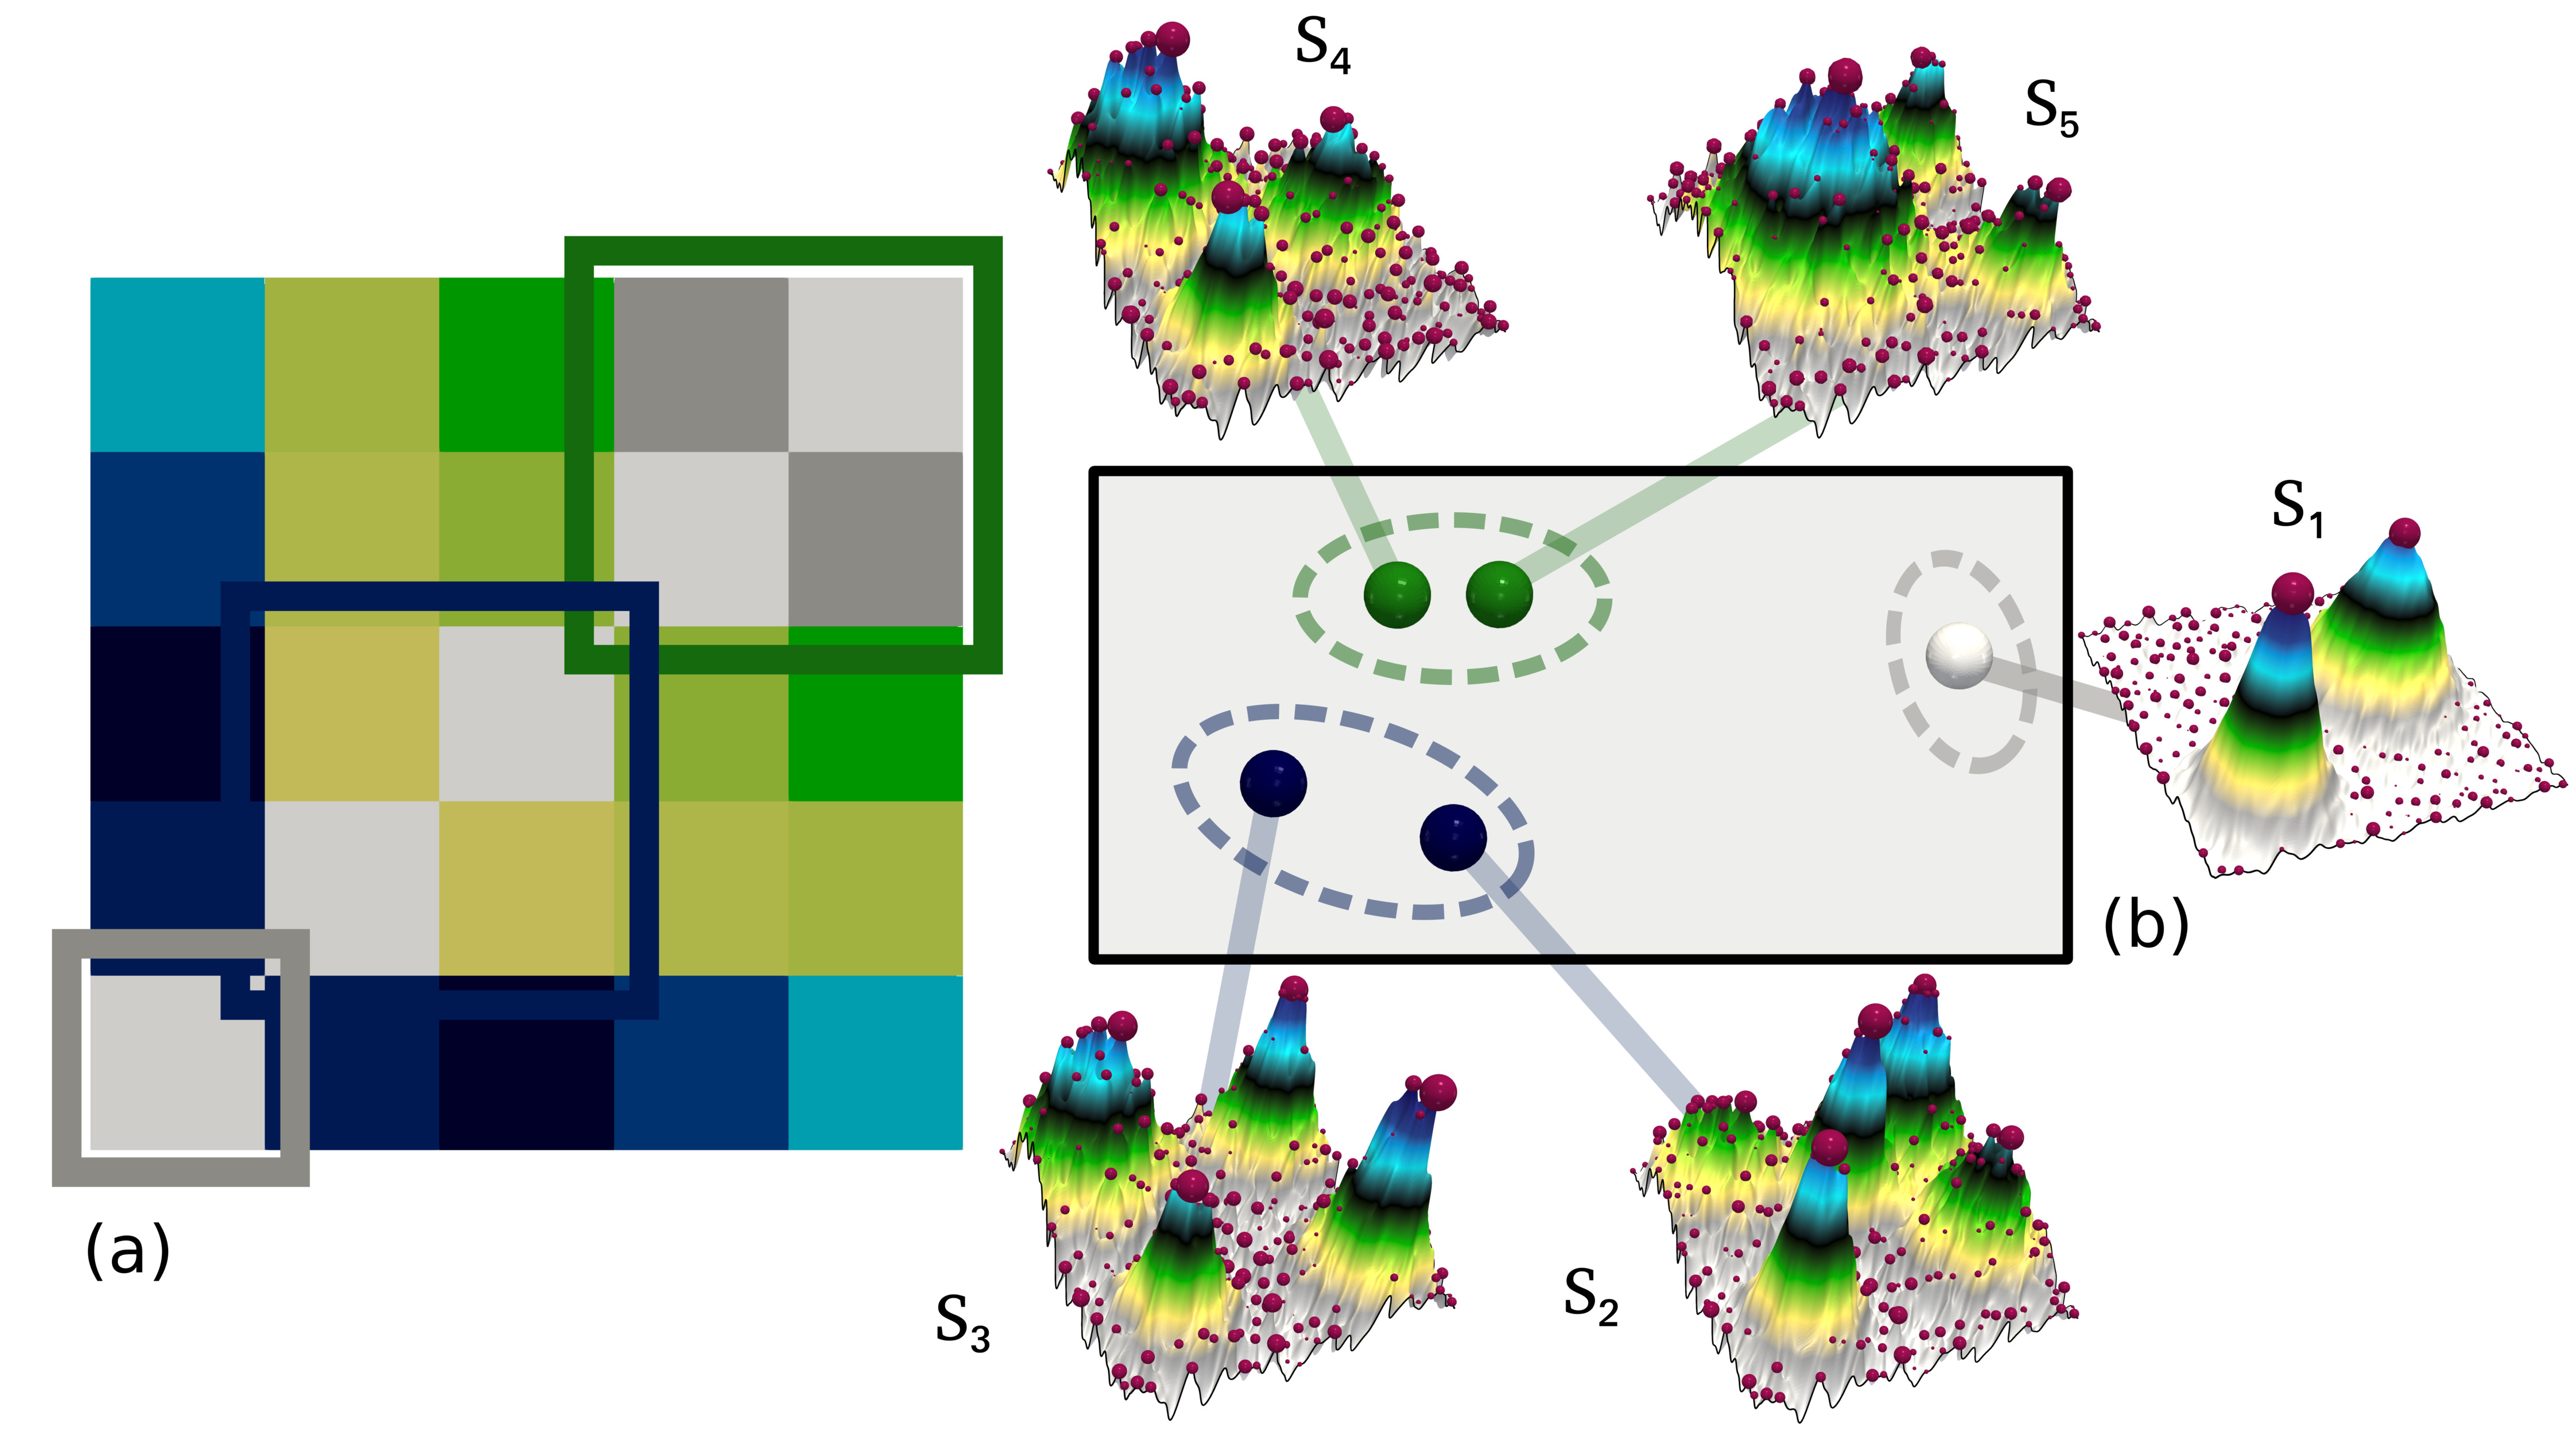
\includegraphics[width=\figureShrink\linewidth]{chapter4_topology_data_analysis/pictures/gaussian_cluster.jpg}
 \mycaption{
 Wasserstein distance matrix for five inputs $S_1$, $S_2$, $S_3$, $S_4$, $S_5$ generated respectively with two, five, for and three Gaussian
functions with different noise levels. Point cloud of the inputs in the Wasserstein distance space colored according to the clusters obtained with the k-means clustering method. We can see that each terrain in a cluster has the same number of Gaussian and level of noise.}
 \label{gaussian_cluster}
\end{figure}
\begin{figure*}
 \centering % avoid the use of \begin{center}...\end{center} and use \centering
 
\includegraphics[width=\figureShrink\linewidth]{chapter4_topology_data_analysis/pictures/KHI_courbes.jpg}
 \mycaption{
Schemes (left) and order (right) studies.
% , left orders study.
Average
persistence curves for 5 configurations with variations of : a (WENO-Z,5), c
(WENO-Z, 7), f (WENO-Z, 5), h (TENO,5). (b,g) persistence curves at $t_0$ (top),
$t_1$ (middle), $t_2$ (bottom).
 Vertical lines on the curves correspond to critical points of small (left) and
high (right) persistence.
% critical points (left) and high persistence (right).
(d,e) Integral differences (grey area) between average persistence curves for
all variations.}
\vspace{2ex}
 \label{curv}
\end{figure*}

\begin{figure*}
 \centering
 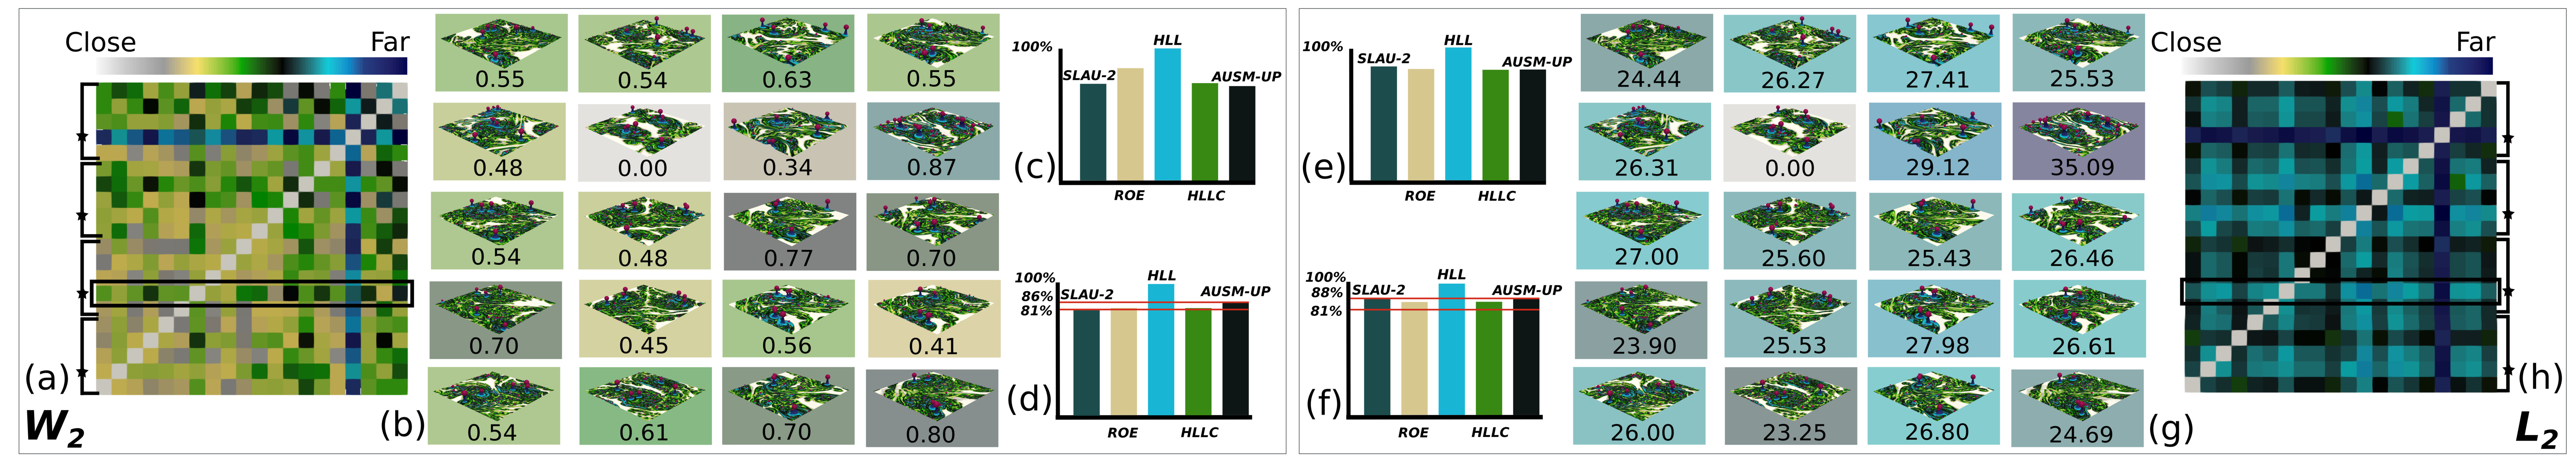
\includegraphics[width=\figureShrink\linewidth]{chapter4_topology_data_analysis/pictures/KHI_distance_to_the_rest.jpg}
 \mycaption{Comparison between the $\wasserstein{2}$ metric (left) and the standard $L_2$-metric (right) for isolating the HLL solver.
 (a,h) Distance matrix for 20 configurations at $t_2$ at $512 \times 512$. Black frames represent the distance between the TENO 7$_{th}$ order with the HLL (matrix lines marked by $\star$) and the other configurations (b,g). Histograms (c,e) are respectively the percentage average of the sum distance matrix of (a,h). Histograms (d,f) are respectively the percentage of the sum distance for all variations.}
 \label{fig_KHIdistance}
\end{figure*}


\subsection{Outlier distance profile}
\label{sec_outlier}
With this protocol (illustrated on toy examples,
\autoref{gaussian_distance}), we want to validate hypothesis H3 (\autoref{Hypotheses}), which means that for all the simulation configurations the HLL solver will be very different from other solvers to describe the Kelvin-Helmholtz instabilities. For this protocol, we take 5 simulation configurations where we fix the reconstruction (TENO or WENO-Z), the physical time ($t_0$, $t_1$, $t_2$), the mesh ($256\times 256, 512\times 512, 1024\times 1024$), the order (5 or 7) and we vary the solvers. The 5 different computations describing the same turbulent flow obtained with the solvers (HLL, SLAU2, AUSM$^+$-UP, HLLC and Roe) are analyzed regarding to the enstrophy.

A distance is used to compare the topology of the enstrophy. Many methods can be used to compute such a distance but in this protocol we focus on 2 metrics: the $L_2$-norm distance directly on the values of the enstrophy and the Wasserstein distance on the persistence diagrams. One can inject other distances if needed. For the Wasserstein, the saddle-maximum persistence diagram is computed on each result. Then, they are grouped in a unique dataset to compute a persistence diagram distance matrix (\autoref{gaussian_distance}). For the $L_2$-norm, a distance matrix  is also created where a line corresponds to the distance in the enstrophy field from one solver to the others.





Thus, the sum of the distances from one solver to the others is computed by
summing the distances on one line of the matrix. The total distance of one 
solver to the others, for all configurations, is simply the sum of all these sum 
distances for every line of the matrix which correspond to the same solver. We 
finally obtain one global distance per solver for all configurations. Finally 
the difference between the distance of the HLL and the distance of the maximizer 
(the second value if HLL is the maximum) gives a separation score. If the
difference is positive, then hypothesis H3 is verified whereas it is not if 
negative, because it means that another solver generates a flow topologically 
more different than the HLL. 
With this protocol, best separations are obtained for high absolute values.
% of 
% the score.

% the higher is the absolute value of the score, the 
% better the separation is.
% with this protocol.



\subsection{Unsupervised classification}
\label{sec_unsupervised}


With the last protocol (illustrated on toy examples in \autoref{gaussian_cluster}),
we want to validate hypotheses H4 and H5 (\autoref{Hypotheses}). We want to verify that the
simulations with the Roe and HLLC solvers are topologically close (hypothesis H4) and the
simulations with the AUSM$^+$-UP and SLAU2 solvers are topologically close (hypothesis H5). To do so, three clustering methods will be used based on Wasserstein distances and the L$_2$- norm(\autoref{sec_topology}).

For the first two clustering methods, we start by computing distance matrix with the protocol of the outlier distance profile \autoref{sec_outlier} using successively the Wasserstein distance and $L_2$-norm matrices (\autoref{gaussian_cluster}a). We apply a dimension reduction to project the distances of the matrix according to 2 components (\autoref{sec_topology}). This projection is used to generate clusters of the matrices with a k-means algorithm (\autoref{sec_topology}) as illustrated on \autoref{gaussian_cluster}b. The third clustering method uses directly the persistence diagrams(\autoref{sec_topology}) without using the distance matrix. All the persistence diagrams are merge into a single dataset to compute the Wasserstein distances between each diagram. The barycenter of persistence diagram is then used to directly compute a cluster, without dimension reduction, in the Wasserstein metric space \cite{vidal_vis19} with the ${W_2}$ distance. Then a k-means algorithm (\autoref{sec_topology}) is applied. 

With these three classification methods, we obtain different associations of our configurations. Each association is going to be scored with a measure of similarities between the clusters regarding to a reference cluster using the Rand Index \cite{rand1971objective}. This Rand index has a value between 0 and 1, with 0 indicating that two clusters do not agree on any pair of points and 1 indicating that the data clusters are exactly the same. Based on the properties of the solvers used in the simulation code HYPERION and detailed in \autoref{sec_solvers}, we define our reference cluster such that the first partition contains the AUSM$^+$-UP and SLAU2 solvers, the second partition the HLLC and Roe solvers and the third partition the HLL solver. The Rand Index is computed for each configuration and averaged per clustering method.
This
% metric
enables the
% precise
ranking of
% allows us to precisely rank
the different solver
behaviors.
% of our solvers.
If the average Rand Index score is close to 1 then both hypotheses H4, showing similarity between the AUSM$^+$-UP and SLAU2 solvers and H5, showing the isolation of the HLL solver, are verified.














\section{Results}
\label{sec_experimentalResults}
This section presents our experimental results and their interpretations, for
the protocols presented in \autoref{sec_protocols}, applied on the ensemble data
described in \autoref{sec_caseStudy}
% , which has been made
(publicly
available \cite{data}).


\subsection{Persistence curve study}



We applied protocol 1 using the persistence curves, on our ensemble dataset of Kelvin-Helmotlz instability (KHI) to verify the hypotheses of separation of the schemes (H1) and the independence of the orders (H2)(\autoref{Hypotheses}). 
The input parameters are setup as detailed in \autoref{sec_protocols}, generating 36 studies. The terrains and curves on
% Figure
\autoref{curv} illustrate the result for one configuration with a 5th order WENO-Z (\autoref{curv}.a), a 7th order WENO-Z (\autoref{curv}.c), a 5th order WENO-Z (\autoref{curv}.f) and a 5th order TENO (\autoref{curv}.h). For the scheme comparison, most of the averaged persistence curves for the TENO schemes (blue curves on \autoref{curv}g) are above the WENO-Z curves (green curves on \autoref{curv}g).
The integral difference, between the average curves, obtain results between $[-5.6,5.2]$ (\autoref{curv}.e), which demonstrates differences on the topology of the enstrophy between the interpolation methods as expected.
Hypothesis H1 is verified on the KHI ensemble dataset. For the study on the 
independence of orders, we see that the averaged persistence curves are often 
close (\autoref{curv}b). However the integral differences obtained for this 
study show larger values for the WENO-Z, \emph{i.e} in between $[-0.5, 8.1]$ 
(\autoref{curv}.d). This analysis highlights that orders play a more important 
role, in terms of topology of the vortices, for WENO-Z than for TENO. Moreover, 
we observe that this difference tends to increase at $t_2$ for both studies 
confirming that the flow is composed of a larger number of vortex as the 
simulation evolves. Hypothesis H2 is verified for the TENO solvers but not for 
the WENO-Z
% as discussed
% later 
% in
(\autoref{insights}).
 



\subsection{Outlier distance profile study}
\label{sec_KHIdistance}


% In order t
To verify the HLL isolation states in hypothesis H3 (\autoref{Hypotheses}) on our ensemble dataset, we implemented our protocol 2 (\autoref{sec_protocols}) based on the Wasserstein distance and the $L_2$-norm (\autoref{sec_topology}). For this study we apply protocol 2 where the time and the resolution are fixed. The parameters that vary are the schemes ($\times 2$), the orders ($\times 2$) and the solvers ($\times 5$) (\autoref{tab_parameters}) thus generating 20 cases. All the distances have been computed according to the protocol of the outlier distance profile. These distances are represented by a global distance matrix where a line represents the 20 configurations (Wasserstein \autoref{fig_KHIdistance}.a and $L_2-$norm \autoref{fig_KHIdistance}.h) compared to a the HLL solver choosen as the reference. The matrix view of \autoref{fig_KHIdistance}b and \autoref{fig_KHIdistance}g show the KHI terrains and the distances of all configurations to the HLL solver.

The study has been done for all time steps and all resolutions generating nine
$20\times 20$ 
distance matrices, for each distance. The histograms (Figs. 
\ref{fig_KHIdistance}.c and \ref{fig_KHIdistance}.e) 
% (\autoref{fig_KHIdistance}.c) and (\autoref{fig_KHIdistance}.e) 
show the average 
of these nine distance matrices for the Wasserstein distance and the 
$L_2$-norm, expressed in terms of percentage according to the distance of HLL 
to the other solvers (HLL being the reference at 100\%). In this case the 
percentage difference in distances to HLL are about 18\% 
(\autoref{fig_KHIdistance}.d) for the Wasserstein and 13\% for the $L_2$ 
(\autoref{fig_KHIdistance}.f). These large percentages confirm that HLL is a 
solver that behaves differently from others.
% More precisely, a
As it does not take
into account contact discontinuities, the interfaces between the vortices
are much less defined than with the other solvers, resulting in a different
number of vortices. From a physical point of view, this result confirms the 
isolation of HLL in all cases. From a topological point of view, it shows that 
the Wasserstein distance is the best at differentiating the HLL solver from the 
others (the distance gap is always bigger than the $L_2$). For this large study 
of 18 distance matrices $20\times 20$, the hypothesis H3 is verified. 

\begin{figure*}
 \centering % avoid the use of \begin{center}...\end{center} and use \centering
 \vspace{-1ex}
 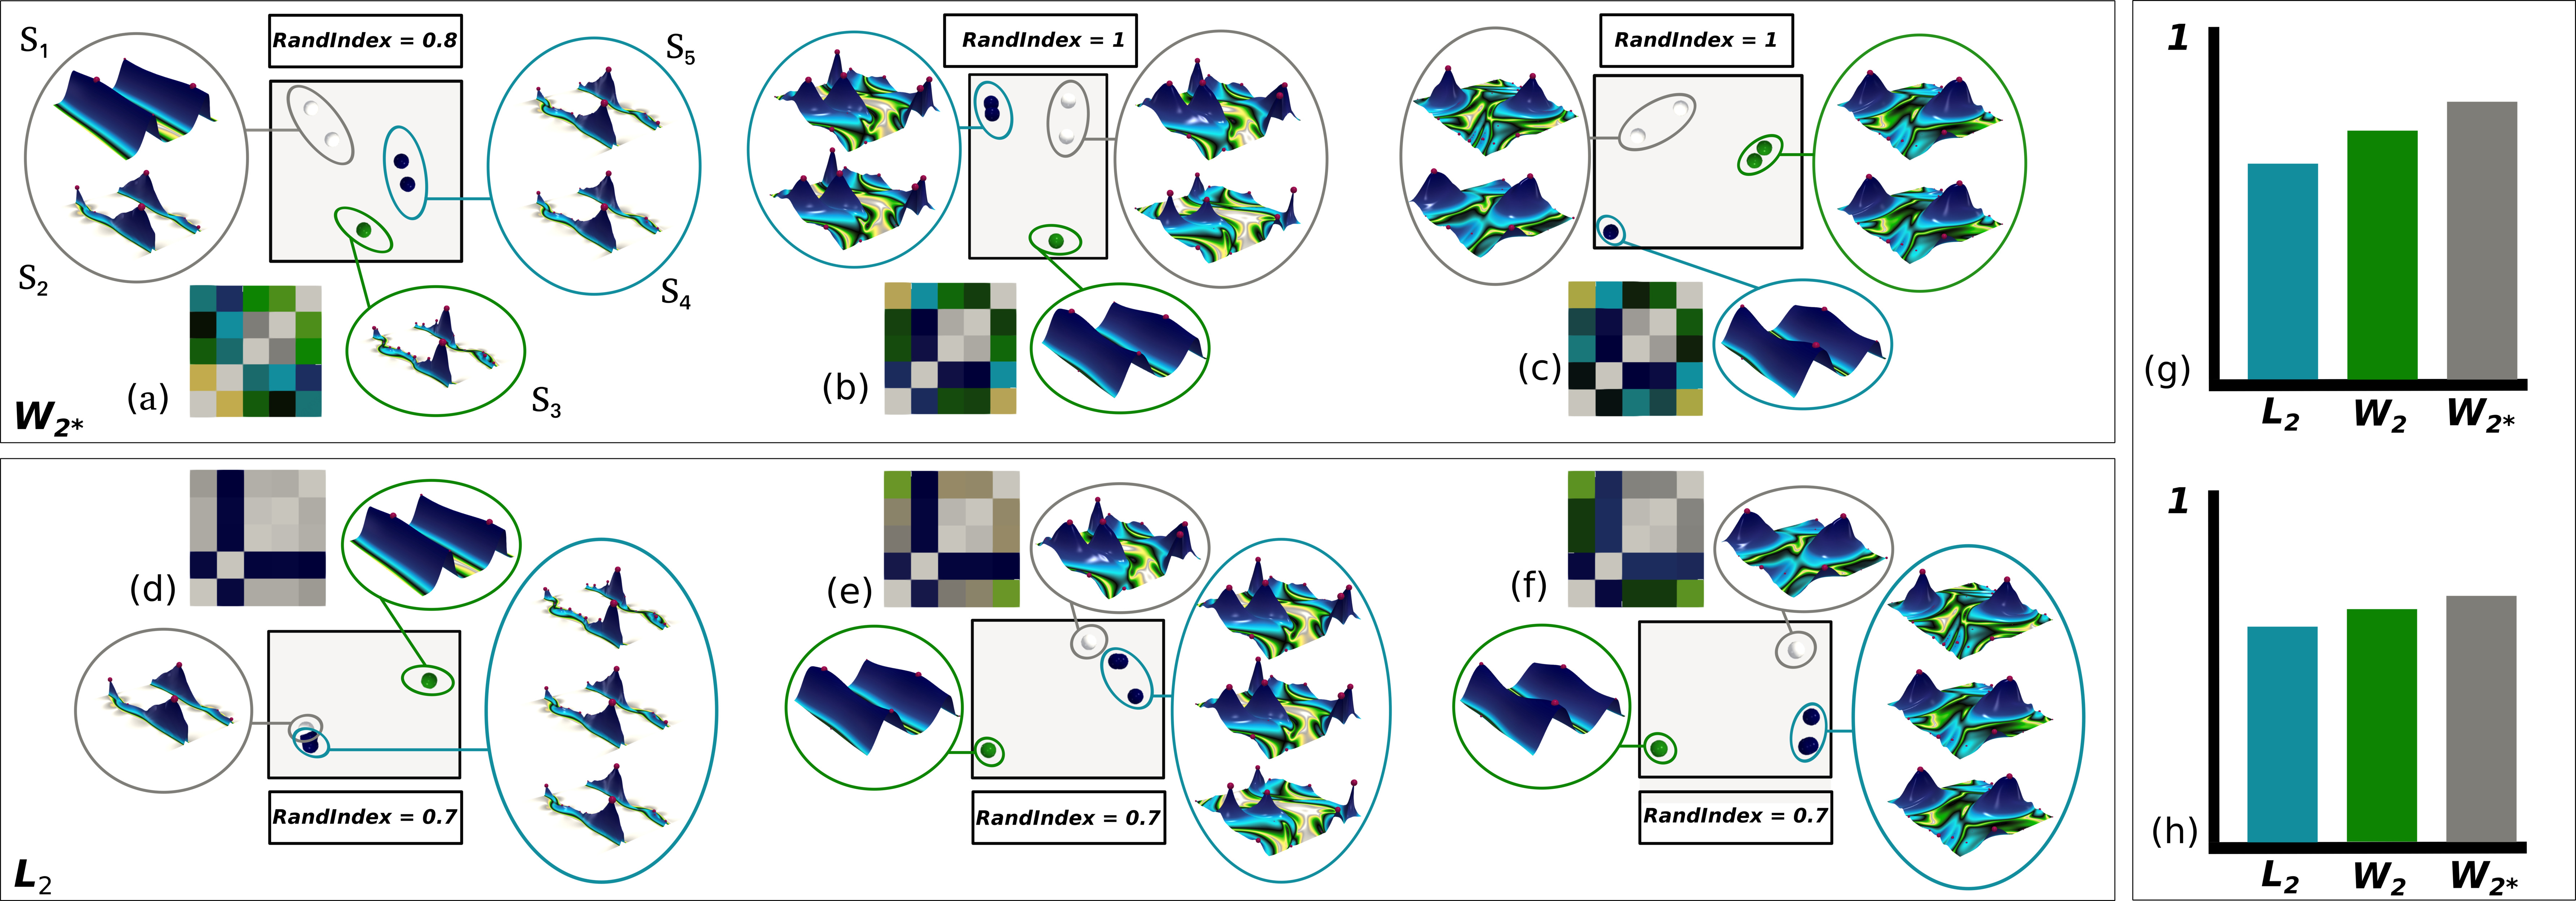
\includegraphics[width=\figureShrink\linewidth]{chapter4_topology_data_analysis/pictures/KHI_cluster.jpg}
 \mycaption{Comparison between the clustering on the Wasserstein metric space \cite{vidal_vis19} (top frame) and a clustering based on the traditional $L_2$ norm (bottom frame) for distinguishing FDS solvers from FTS solvers.
Point clouds at $t_0$, $t_1$,$t_2$ with a first order scheme at $256\times 256$.
The point cloud is a representation of the five scalar-fields in the distance
space colored according to the clusters obtained. The Rand Index are computed
with the five configurations $S_1$ (SLAU2), $S_2$ (HLL), $S_3$ (AUSM$^+$-UP),
$S_4$ (Roe), $S_5$ (HLLC). (g,h) Average Rand Index for all variations for the
high orders (bottom) and the first order (top).}
\label{fig_khi_cluster}
\end{figure*}


\subsection{Unsupervised classification study}
 \label{sec_khi_cluster}
To improve our understanding on the behavior of the solvers into our simulation code, we implemented protocol 3 on the unsupervised classification (\autoref{sec_protocols}) to verified the hypotheses H4 and H5 (\autoref{Hypotheses}). The goal is to identify the separation of FDS type solvers from the FTS type solvers (\autoref{sec_solvers}). We are interested in the low Mach reconstructions (\autoref{sec_solvers}). The challenge comes from the fact that small vortices are reconstructed on only a few cells. So, we implemented protocol 3 with the distances and clustering method detailed in \autoref{sec_protocols} leading to 5 simulation configurations (\autoref{tab_parameters}) with variable solvers. To focus on the small vortices we used a threshold of 0.38 persistence for the topological methods. On the KHI ensemble, we generated 36 clusters from the threshold persistence diagrams and obtain the Rand Index for all of them. \autoref{fig_khi_cluster}.a, \autoref{fig_khi_cluster}.b, \autoref{fig_khi_cluster}.c show the $W_2*$ clustering for the three timesteps and \autoref{fig_khi_cluster}.d, \autoref{fig_khi_cluster}.e, \autoref{fig_khi_cluster}.f for the $L_2$.

Histogram \autoref{fig_khi_cluster}.h shows the average Rand Index for the 
three methods with a value of 0.63 for $L_2$, 0.66 for $W_2$ and 0.71 for $W_2*$.
There is very little difference between the topological and geometric results 
and each of the methods struggles to get the right cluster. Hypotheses H4 and H5 
are not verified for high orders. However, to highlight the differences between 
solvers, it is necessary to use a reference reconstruction that barely captures 
small scale turbulence due to order dissipation (\autoref{sec_solvers}).
Thus, we applied protocol 3 (\autoref{sec_protocols}) on a more restricted 
dataset at order 1. Histogram \autoref{fig_khi_cluster}.g shows the average 
Rand 
Index at order 1 with the three methods leading to 0.63 for $L_2$, 0.71 for $W_2$
and 0.78 for $W_2*$. In this case, we notice that for any reconstruction, the 
topological methods obtain better clustering. Moreover, the study with order 1 
shows that the $W_2*$ method enhances solver isolation.
% of the solvers.
With this
high score of the Rand Index hypotheses H4 and H5 are verified with the first 
order. 

\subsection{Unanticipated insights}
\label{insights}

During the analysis of the persistence curves generated by our protocol 1, we found significant differences on the topology of the enstrophy between the orders for the WENO-Z. By increasing the order, we increase the accuracy of our calculation that generates more structures into the turbulent flow. On the other hand, there is no difference between the orders obtained with the TENO. This means that other ingredients in the TENO reconstruction play an important role in the computation of the turbulence such as the separation of the scales. In addition, the persistence curves also allowed us to observe that the WENO-Z schemes produce more numerical errors than the TENO. As presented in \autoref{sec_khi_cluster}, H4 and H5 hypotheses have not been verified for high orders. This means that the topological analysis does not capture the differences between the solvers. This may be due to the reconstructions which are accurate enough to calculate all velocities in the Kelvin-Helmholtz instability. 

\subsection{Limitations}
As discussed in \autoref{sec_KHIdistance}, in comparison to the $L_2$ norm, the Wasserstein distance
improvesthe separation of the HLL solver, but only by $5 \%$ (distance difference percentage). While this improvement may seem marginal, we would like to stress its significance given such challenging data,in particular with regard to the traditional approach based on kinetic energy, shown \autoref{energie}, where the five solvers can hardly be distinguished from each other.

Similarly, we can see that the Rand Index score for the three clustering
methods detailed in \autoref{sec_khi_cluster} are quite close to each other as
illustrated on \autoref{fig_khi_cluster}.h. These close scores are due to the 
interpolations schemes (\autoref{sec_simulation}) which cover up the differences 
between the different solvers.
In other words, the variations in vortex distributions induced by the choice of solver are too subtle, given the importance of the interpolation order on the outcome. As shown in \autoref{fig_khi_cluster} (top), we were still able to overcome this limitation by considering a
reconstruction that is not dedicated to turbulence, \emph{i.e.} an upwind scheme 
of order 1. This enabled us to exaggerate the impact of the solvers, thereby allowing us to
validate hypotheses H4 and H5 as reported in \autoref{sec_khi_cluster}.



\section{Conclusion}
In this paper, we have presented an experimental protocol for the comparison of
numerical methods on a Kelvin-Helmholtz instability using topological analysis.
An ensemble dataset of 180 members has been computed for this instability by a
simulation code developed in our institution and running on a supercomputer.
While traditional approaches based on the kinetic energy (\autoref{energie}) only enable
to validate the physical conformity of the generated flow,
% to assess the physical conformity of the generated flow,
our overall approach provides finer analyses. In particular,
% Based on the assumptions made in the literature (\autoref{sec_simulation}),
the
protocol using the persistence curves (\autoref{sec_persistence}) allowed us to
observe differences between the TENO and WENO-Z reconstructions. It also
confirms an independence of the
reconstruction order (5 or 7) when
using the TENO scheme allowing
% speedup
practical
computational speedup,
without loss of precision. The protocol
based on the Wasserstein distance (\autoref{sec_outlier}) succeeded in
discriminating the HLL solvers from other configurations, validating the use of
such a topological analysis to confirm domain field expectations. The last
protocol, based on recent clustering methods (\autoref{sec_khi_cluster})
successfully differentiates the topology of computations based on FDS (Flux
Difference Splitting) and FTS (Flux Type Splitting) solvers.
Overall, the validation of the hypotheses reported by CFD experts (\autoref{sec_hypotheses}) provides reliable indications for the tuning of a flow simulation, to help CFD users achieve the best balance between computation accuracy and speed.
%
%
% in contrast to traditional approaches (\autoref{energie}), which only validate the physical plausibility of a flow, our framework enabled the validation of the above hypotheses (formalized in \autoref{sec_hypotheses})}
% In particular, the validation of these hypotheses are a practical contribution towards }
% Flux Differe
% (FDS) and FTS solver computations.


The results obtained in this experimental study also show
the viability of topological methods for the representation and comparison of
Kelvin-Helmholtz
instabilities.
%
% that
%
% we can take confidence in the topological treatment for a Kelvin-Helmholtz
% instability.
The interesting aspect of these topological protocols is that the
numerical method comparisons are based on physical differences rather than on
unreliable, low-level, pointwise measures.
% quantitative.
The direction we wish to take now, for our future work, is
the extension of these protocols to 3D datasets of external hypersonics aerodynamics.
% However, in order to isolate one phenomenon on 3D data, a
% threshold study will have to be implemented. It will be necessary to decide
% which phenomenon we want to observe, such as boundary layer turbulence or
% vortices generated at the back of the hypersonic vehicle.
Another direction we
want to investigate is the evaluation of other tools used in the protocol such
as new topological distances \cite{pont_vis21} or clustering methods. Finally, this experimental
study allows us, with confidence, to consider applying these protocols to other
hydrodynamic turbulent flows studied in our institution in the domain of
hypersonic vehicle design.


% \section{Acknowledgments}
%future work:
%benchmark for other topological comparison methods.



\end{document}

